\documentclass[letterpaper,12pt]{article}
\usepackage[margin=1in,includehead]{geometry}
\usepackage{parskip}

\usepackage{amsmath}
\usepackage{bm}
\usepackage{amssymb}

\usepackage{float}
\usepackage{graphicx}
\usepackage{microtype}
\usepackage{enumitem}
\setlist{nosep}

\usepackage{minted}

\usepackage{natbib}
\bibliographystyle{plainnat}
\renewcommand{\bibsection}{\section{\bibname}} %make bibliography show in TOC
% \usepackage{backref}
\usepackage[backref=page]{hyperref}
\usepackage{libertine}
\usepackage[libertine,cmintegrals,cmbraces,vvarbb]{newtxmath}
\usepackage[scaled=0.95]{inconsolata}

% change the format of the 'cited on'
\usepackage{etoolbox}
\makeatletter
\patchcmd{\BR@backref}{\newblock}{\newblock[Cited on pg.~}{}{}
\patchcmd{\BR@backref}{\par}{]\par}{}{}
\makeatother

\usepackage{doi}

\usepackage{siunitx}

\renewcommand{\listingscaption}{Code Snippet}

\usepackage[font={small},labelfont={bf,it},textfont={it}]{caption}

\renewcommand{\footnoterule}{\vfill\kern -3pt \hrule width 0.4\columnwidth \kern 2.6pt}

\usepackage{relsize}
\AtBeginEnvironment{quote}{\smaller}

\usepackage{fancyhdr}
\pagestyle{fancy}
\fancyhead{}
\fancyhead[L]{\rightmark}
\fancyhead[R]{\thepage}
\fancyfoot{}


\setcounter{tocdepth}{2}

\title{Aggregating experiments}
\author{Anthony Ozerov}
\date{\today}



\begin{document}

\maketitle

\begin{abstract}
\noindent Many applied studies seek to aggregate multiple estimates of a target quantity $\theta$ from different experiments/methods, taking into account both systematic errors (or, generally, between-study heterogeneity) and within-study noise. Inference typically involves strong assumptions, such as a normal random-effects model. We develop new methods with weaker assumptions by drawing on nonparametric statistics. To evaluate the assumptions and performance of different methods, we use real-world physical science datasets with and without ground truths and perform a simulation study. The nonparametric methods perform favorably in these analyses, and we also find that an additive as opposed to multiplicative error model is appropriate. We present case studies to illustrate the careful application of meta-analysis in the physical sciences.
\end{abstract}

\newpage

\tableofcontents

\newpage

\section{Introduction}\label{introduction}

Combining multiple estimates of a quantity into one is common across the sciences. In medicine and the social sciences, meta-analyses find studies/experiments which estimate the same quantity (e.g.~the treatment effect of a medicine) and combine them into one estimate, with associated uncertainties. In Earth science, ``intercomparison'' studies take models from different teams and study their differences, sometimes attempting to reconcile them and produce one better estimate. In physics, the values of fundamental constants and measuremnets of fundamental particles obtained in different experiments must also be somehow reconciled.

One key issue that arises is systematic uncertainty, where an estimate of a quantity may have some error not due to noise which can't be reduced by collecting a larger sample or running the experiment for longer. This error can be due to issues in the experiment like a non-randomly-sampled population, or an instrument which is miscalibrated, or analysis issues like approximations and model imperfections. Empirically, this can be seen when results from different experiments/teams/methods are far outside of each other's error bars. Aggregating multiple estimates must therefore not only account for the modeled noise, but also somehow model the systematic uncertainties in the different estimates. This leads to the counterintuitive fact that combining multiple estimates sometimes \emph{increases} our uncertainty, rather than decreasing it---this is because the level of systematic error is not apparent in only one estimate, and becomes apparent when we see more.

We will begin in this section by discussing and setting up the general problem. Then, in Section \ref{sec:methods}, we will go through different sets of assumptions which can be used to do inference in this setting, and follow in Section \ref{sec:assumptions} with an evaluation of the assumptions using real-world datasets. Informed by the results of Section \ref{sec:assumptions}, we will perform a simulation study in Section \ref{sec:simulation} to evaluate the performance of different inference methods and their sensitivity to violations of assumptions. This will be followed by Section \ref{sec:realworld}, where we will investigate the performance on real-world datasets.

We will present results on two toy examples---estimates of the gravitational constant and of the Planck constant---to illustrate how the different methods work when applied to real data. Finally, we will present two case studies: aggregating estimates of the properties of fundamental particles, and aggregating estimates of Antarctic ice sheet mass loss over time. This will illustrate how the methods presented and discussed here can be used in real scientific problems.


\subsection{Thought experiment}\label{thought-experiment}

Suppose you are given a jar containing a lot of jelly beans, and you want to get an idea of how many jelly beans it contains without counting. You ask five of your friends to try to figure it out, and they give you the following numbers:

\begin{itemize}

\item
  Friend A: 540
\item
  Friend B: 535
\item
  Friend C: 556
\item
  Friend D: 543
\item
  Friend E: 637
\end{itemize}

You want to make an interval that has a roughly 70\% chance of containing the true number of jelly beans. What are some reasonable intervals?

\begin{itemize}

\item
  $[535, 637]$: You think Friends B and E are both smart people with reasonable estimates, and probably the true value is not outside the range of all the estimates.
\item
  $[535, 556]$: You think Friend E is probably overestimating, as your other smart friends are all clustered together.
\item
  $[100, 1000]$: Maybe all of your friends are way off! They could all be underestimating or overestimating the number together if they used a similar approach or suffer from the same bias.
\end{itemize}

Here are some things you may consider when picking an interval:

\begin{itemize}

\item
  Are all of the estimates good, reasonable estimates? Should we discard any? To help decide, you may want to interrogate the methods that your friends used. If Friend E's method looks good, should you do something to resolve the large discrepancy in results with the others?
\item
  How diverse were the methods used? If they all used the same, wrong method then they might all be very wrong. On the other hand, if they all used different methods and arrived at similar results, you may be more inclined to trust them.
\item
  Do the methods of each friend yield values which are centered around the truth?
\item
  Were there any social factors? For example, if Friend D publicly announced their result and is highly respected among the others, the others could have been disinclined to give highly discrepant results.
\end{itemize}

Evidently, combining these five estimates into an interval is not a trivial matter. Indeed, without knowing a lot more details about how the estimates came about from the truth and are related to each other, it will not be possible to design a statistical method to yield a confidence interval or credible interval with the desired probability.

Now, imagine each of your friends also gave a standard deviation associated with their estimate. This would, in fact, complicate the situation further, as we would need to ask the following questions:

\begin{itemize}

\item
  What do the standard deviations mean?
\item
  Which distributions are they the standard deviations of? Do the numbers and the standard deviations together completely describe the distributions?
\item
  Are the distributions frequentist sampling distributions or Bayesian posterior distributions?
\item
  Do the standard deviations account for just statistical noise involved in their method, or some or all parts of their systematic biases?
\end{itemize}

If there is any heterogeneity among the friends in the answers to these questions, our task will become even more complicated. What do we do if Friend A's standard deviation is for just statistical noise but Friend B's also tries to take into account systematic error?

\subsection{Setup}\label{setup}

Suppose we are given $n$ estimates $y_1,\ldots,y_n$ of a number $\theta$, from $n$ experiments or teams or methods. It is possible that each of these estimates has error from two sources: \textbf{systematic} and \textbf{statistical} (i.e.~noise). (For instance, we can have a data-generating process where $y_i$ is actually a noisy estimate of $\theta_i$, which is what experiment $i$ would see if it had no noise; because of systematic error, in general $\theta_i\neq \theta$).

Suppose we are further given a standard deviation $\sigma_i$ for each $y_i$. Experimenter $i$ believes that $\sigma_i$ is a good estimate for the uncertainty in $y_i$ due to noise.

In this setting, how can we learn something about $\theta$? Without making any assumptions, we can't learn anything (for instance, we could have $\theta_i=\theta-a\ \forall i$, in which case we are unable to recover $\theta$ without knowing something about $a$).

This is the problem we will consider in this paper. In some cases, we will suppose that we are not given $\sigma_i$'s. But for simplicity we will suppose being given no more than $(y_i,\sigma_i)$ pairs: no asymmetric uncertainties, no full predictive distributions, and no breaking down of $\sigma_i$ into multiple components.

\subsection{History}\label{sec:history}

The core statistical methods to aggregate data from different observations, and eventually different studies, developed first in the physical sciences. The method of ``least-squares'' (i.e., minimizing the sum of squared residuals to obtain a best-fit) was hinted at in the context of astronomy by Roger Cotes in his posthumously published \emph{Opera Miscellanea} \citeyearpar{cotes1722opera}.\footnote{He described that to calculate the position of an object from several observations with different errors, one must take the center of the positions as weighted by the inverse of the ``limits of the errors.'' This is the original text:
  \begin{quote}Ad eundem fere modum in aliis casibus Limites inveniuntur Errorum qui ex minus accuratis observationibus ortum ducunt, quin \& Positiones ad Observandum commodissimae deprehenduntur: ut mihi vix quidquam ulterius desiderari videatur postquam ostensum fuerit qua ratione Probabilitas maxima in his rebus haberi possit, ubi diversae Observationes, in eundem finem institutae, paullulum diversas ab invicem conclusiones exhibent. Id autem fiet ad modum sequentis Exempli. Sit p locus Objecti alicujus ex Observatione prima definitus, q, r, s ejusdem Objecti loca ex Observationibus subsequentibus; sint insuper P, Q, R, S pondera reciproce proportionalia spatiis Evagationum, per quae se diffundere possint Errores ex Observationibus singulis prodeuntes, quaeque dantur ex datis Errorum Limitibus; \& ad puncta p, q, r, s posita intelligantur pondera P, Q, R, S \& inveniatur eorum gravitatis centrum Z: dico punctum Z fore Locum Objecti maxime probabilem, qui pro vero ejus loco tutissime haberi potest.
  
  \hfill-- \citet[Aestimatio Errorum in Mixta Mathesi, pg. 22]{cotes1722opera}\end{quote}}
Astronomy was indeed a core motiving science for these developments through the 19th century. The simple observational problem of recording the position of an object (say, a planet or asteroid) across multiple days, then computing its orbit, requires combining multiple noisy estimates. Least squares was formalized by \citet[art. 179]{gauss1857theory} and stated in a more recognizable, modern form for simple one-dimensional experiment- or observation-aggregating by \citet[art. 69-71]{airy1861algebraical}. Effectively, this was the Fixed Effect model and method described below, which does not account for any systematic error not modeled by the given $\sigma_i$'s.

As early as 1881, we see FW Clarke, a chemist, using least-squares to aggregate measurements of atomic weights reported by different experimenters who used different methods \citep{clarke1881abstract}. What is lacking from Clarke's work, though, is a statistical evaluation of systematic errors---we see several weighted means with quoted uncertainties that are far too low when considering the spread of the different experimenters' results.\footnote{Consider the following results quoted for the atomic weight of chromium:
  \begin{quote}
    The data studied were by Berlin, Moberg, Lefort, Wildenstein, Kessler, and Siewert. General mean from all, Cr=52.453; $\pm$.015. Berlin's work, considered by itself, gives Cr=52.389; $\pm$.019. Siewert's results give Cr=52.009; $\pm$.025. I regard-the last value as freest from constant errors, and use it in subsequent calculations.
  
    \hfill-- \cite{clarke1881abstract}
  \end{quote}
}

In fundamental physics, statistical meta-analysis can be traced back at least as far as \cite{burgess1902value}, which calculated the error-weighted mean of the gravitational constant $G$. This work suffered from similar issues as Clarke's atomic weights. Finally, \cite{birge1919most} calculated an error-weighted mean of several determinations of Planck's constant $h$ obtained from different experiments. Again, this was under the Fixed Effect model. What goes beyond a simple error-weighted mean, though, is Birge's discussion of systematic uncertainity. In particular, he computed the residuals of each result from the error-weighted mean, and compared those residuals to the given errors $\sigma_i$. He concluded that the results were ``consistent'' \cite{birge1919most}. Thus he provided a quantitative evaluation of the presence of systematic error or underestimation of the experiments' uncertainties.

By the early 20th century, measurements and estimates of various physical constants were becoming increasingly numerous. These physical constants were also key to the work of the experimental physicist, whose experimental results involved calculations with these uncertain physical constants, or were even stated \emph{in terms of} them (as they entered somewhere into the units). Comparing and discussing different results thus became increasingly difficult as physicists did agree on one set of values. Therefore, by 1929, Birge set out to collate different experimental results and produce a ``self-consistent'' set of constants based on all readily available measurements (since many constants are functions of one another, the values for a set of constants need to be internally consistent, which introduces additional difficulties).\footnote{It appears that the first work performing a least-squares adjustment of multiple physical constants at once may be \cite{harkness1891solar}. However, Harkness does not perform sophisticated statistical aggregations of the experiments contributing to each constant: he uses either simple arithmetic means or picks one of the results.} Such a collation/aggregation of results has come to be known as an ``adjustment.''

In Birge's pioneering work \citeyearpar{birge1929probable}, it is apparent that much of the difficulty lay in interpreting the uncertainties which experimental results reported in diverse ways:
\begin{quote}
  One of the greatest difficulties in the present work has been the proper weighting of various results, one of which is stated in terms of ``limit of error,'' another in terms of a ``probable error,'' another possibly with the error undefined, and still another with no definite statement as to accuracy. This is quite aside from the reliability or correctness of the method used by each investigator in arriving at his stated error.

  \hfill -- \cite{birge1929probable}
\end{quote} 

To perform his ``adjustment,'' Birge used a combination of heuristics and statistics. In terms of heuristics, he used domain knowledge or apparent inconsistency to discard poor or outdated experimental results. From the statistical side, he again used the least-squares method or Fixed Effect model. In the context of aggregating physics experiments, ``least-squares'' has come to mean taking an inverse-variance-weighted mean of the $y_i$'s, where the variances are somehow calculated from the $y_i$'s and $\sigma_i$ (in the simplest case, the variances are taken as $1/\sigma_i^2$, and the weights are proportional to $1/\sigma_i^2$). The uncertainty is taken as appropriate for a weighted mean. But Birge was quick to discard least-squares results when they seemed insensible. For example, in his calculation of the charge of the electron, for which only two values were used, he took a weighted mean as usual, but adopted ``as its probable error the smaller of the two individual errors, rather than that given by least squares, since the latter is rather meaningless when only two observations are concerned'' \citep{birge1929probable}.

By 1932, Birge developed what is now known as the ``Birge ratio'' method for least-squares. The first clear statement of it is in \cite{birge1932calculation}. After obtaining the weighted mean by least-squares as usual, he computes the ratio of the error in a point calculated by its ``external consistency'' (using the residuals between experiments and the weighted mean) to that calculated by ``internal consistency'' (using its own given error, which at the time was often computed empirically from the spread of multiple measurements).\footnote{This ratio is stated in eq.~20 of \citet{birge1932calculation}.} This is a useful quantitative diagnostic tool: if the ratio is large, it indicates that the individual experiments have more spread between them than we would expect from their individual errors. But he goes beyond diagnostics, and, when calculating the error of the weighted mean, he advocates choosing the larger of the ``external consistency'' and ``internal consistency'' errors. This effectively forms the Birge ratio method which will be described more precisely in a later section. However, Birge also writes that when the ratio is large, the errors should be adjusted manually with personal judgment.

As noted by \citet{baker2013meta}, this thread of meta-analysis research in physics seems to have occurred largely separate from the field of statistics. Indeed, \citet{cochran1954combination} discusses the problem of meta-analysis with physical constants as an example, but seems unaware of Birge's line of work.\footnote{
He offers an insightful independent perspective on combining experiments measuring physical constants (note: by ``interaction'' below he means ``an interaction of the effect with experiments''---this is the unaccounted-for variation in experimental results.):
\begin{quote}
  In the determination of a physical constant, we might conclude that interaction exists because some of the experiments (e.g.~the earlier ones) were done by a technique that is subject to a bias of unknown magnitude, whereas the remainder of the experiments appear to be unbiased. In this event we would presumably discard the results from the biased experiments and consider only a combination of results from the unbiased experiments.

  \ldots

  Occasionally, in laboratory experiments which were thought to be well-controlled, large interactions may appear for which no adequate explanation can be given. In this event it might be best to hand the problem back to the experimenters, on the grounds that there is not much point in attempting a ``best'' combined estimate until the experimenters can reach better agreement in their results, or at least find out why they disagree.\hfill --\citet{cochran1954combination}
\end{quote}
}

Aggregations of fundamental physical constants are now performed by the Committee on Data of the International Science Council (CODATA). But this task of aggregating well-defined physical constants has only expanded, and now includes constants for particle properties in the standard model, performed by the Particle Data Group (PDG) in its frequently-updated \textit{Review of Particle Physics}. Both CODATA and the PDG use slight variations on Birge's method. The challenges of dealing with systematic uncertainty are illustrated by PDG's ``History Plots'' \citep[pg. 19, Figure 1]{navas2024review}, which show how, as PDG incorporated new experiments and discarded old ones over time, the resulting estimates of some particle properties have varied outside of the range of their error bars.

An additional task has also arisen with the development of data- and simulation-driven Earth science. This involves estimates of less well-defined (and sometimes in principle unknowable) quantities. For example, we may consider the amount of global warming in the past or future, or the historical and present-day rate of ice mass loss in polar regions. Here, looking at multiple estimates is sometimes known as ``intercomparison.'' Some intercomparison studies simply seek to review the differences in the methods and results, while others seek to statistically combine multiple estimates into one.

\subsection{Experiment aggregating vs.~forecast ensembling}

Our discussion of meta-analysis / experiment aggregation brings us close to a related area: opinion pooling, or ensemble forecasting. Let's compare:

\begin{enumerate}
\item
  In experiment aggregation, we have been discussing a situation where $n$ different experimenters/teams/studies come up with $n$ different estimates $y_1,\ldots,y_n$ for some quantity $\theta$, possibly with associated uncertainties $\sigma_1,\ldots,\sigma_n$.
\item
  In ensemble forecasting or opinion pooling, we may ask $n$ different teams to predict how much rain will fall tomorrow, and maybe they will each give values $y_1,\ldots,y_n$ with associated uncertainties $\sigma_1,\ldots,\sigma_n$.
\end{enumerate}

These seem like very similar situations. So can we use the same methods for both of them?

Let's give an example from paleoclimatology to further explore the difference. It will illustrate that it is not the act of ``forecasting'' (i.e.~predicting something in the future) itself that leads to any difference, but the effectively irreducible uncertainty of the estimand.

\begin{enumerate}
\item
  $\theta$ is the mean global temperature between 10,000 years ago and 11,000 years ago
\item
  $\theta$ is the air temperature at solar noon on January 1, 10,000 BP in what is now Berkeley, CA.
\end{enumerate}

In the first case, different teams may use different historical temperature proxies and come up with different estimates of $\theta$. If they all use different independent datasets (e.g.~different ice cores), then assuming their methods are good we expect them to come back with results $y_i$ clustered around $\theta$. If the methods are good, it would be fairly unlikely for the true $\theta$ to lie above \emph{all} of the $y_i$'s.

In the second case, probably what teams will do is use an answer from the first case, combined somehow with some regional weather variation models. They will each come back with a $y_i$ representing a long-run average and a fairly large $\sigma_i$, because on any given day the temperature can be quite different. If January 1, 10,000 BP happened to be a very hot day in what is now Berkeley, CA, then it is quite possible for the true $\theta$ to lie above \emph{all} of the $y_i$'s.

In the first case, it is possible for the $y_i$'s to be roughly conditionally independent given $\theta$. In the second case, the $y_i$'s will not be conditionally independent given $\theta$. Maybe they will be conditionally independent given a long-term average, but conditioning on the $\theta$ itself does not make them independent---the $y_i$'s will vary above and below $\theta$ together.

How does this inform the way we do aggregation? It may be helpful to take up a Bayesian perspective to understand this difference.

\begin{enumerate}
\item
  In the case of experiment aggregation, we have $n$ different experiments which produce data $d_1,\ldots,d_n$. These data come from likelihoods $p(D_1|\theta),\ldots,p(D_n|\theta)$. Crucially, we think the $D_i$ are independent given $\theta$. The experimenters themselves think the $d_i$ come from $p_1(D_1|\theta),\ldots,p_n(D_n|\theta)$, because they have their own understandings of the likelihood of an observation given the value of $\theta$, due to, for example, distributional approximations or different beliefs about their instruments. Now, suppose all of the estimates we receive from the different experimenters are reflected as Bayesian posterior probabilities for $\theta$, written as distributions $p_1(\theta|D_1=d_1),\ldots,p_n(\theta|D_n=d_n)$.\footnote{The posteriors $p_i(\theta|D_i=d_i)$ will depend not only on the different likelihoods $p_i(D_i|\theta)$, but also on priors $p_i(\theta)$ which may not be the same for different experimenters.} The key is that each experiment created different data, and we want to combine it to obtain something like $p(\theta|D_1=d_1,\ldots,D_n=d_n)$ as our ``aggregated'' estimate for $\theta$. We will expect that, as $n$ increases, our distribution $p(\theta|D_1=d_1,\ldots,D_n=d_n)$ will get narrower.\footnote{This narrowing may only be up to a point. For example, we can consider a situation where we are actually interested in $\theta'=\theta+\varepsilon$, where, say, $\varepsilon\sim\mathcal{N}(0,1)$, but $D_i\perp\!\!\!\!\perp\varepsilon$. In this case, we will always have an irreducible error in our posterior for $\theta'$. As the variance of $\varepsilon$ increases we will actually start to be more in the second ``opinion pooling'' setting, where the different estimates were made with the same information.}
\item
  In the case of opinion pooling or aggregating forecasts, we have $n$ different people who each observe the same state of the world $D=d$. Then, each of them comes up with their own posterior distributions (based on their own priors and likelihood functions), and they report them to us. So we get $p_1(\theta|D=d),\ldots,p_n(\theta|D=d)$. Our task is to somehow combine these into one $p(\theta|D=d)$. Because each forecaster has access to roughly the same data $D=d$, we do not expect our distribution $p(\theta|D=d)$ to get narrower as $n$ increases (though it may become more well-calibrated).
\end{enumerate}

It is extremely important to distinguish which case we are in, as it will lead to different statistical methods being appropriate.\footnote{It may not always be easy to determine which setting we are in. Consider the case of Antarctic ice mass loss, which will be discussed later. If we are estimating how much ice Antarctica lost over the last 20 years, that seems like it lies more in case (1), due to the large amount of independent data sources available documenting this phenomenon over a long time period at a high temporal resolution. How about the ice mass loss on one particular day in the last 20 years? That seems more like (2)---the temporal resolution of our data won't be good enough to do much better than a monthly average with some correction for the day's weather and a wide uncertainty. But if we consider the mass loss on a weekly, monthly, or yearly scale, these must lie somewhere in between the two cases.} In particular, methods for (2) will typically lead to far wider uncertainties than those for (1). For example, suppose $y_1=\ldots=y_n=0$, and $\sigma_1=\ldots=\sigma_n=1$. Under (1) a reasonable estimate for $\theta$ might be $0$ with standard deviation $1/\sqrt{n}$. Under (2) a reasonable estimate for $\theta$ might be $0$ with standard deviation 1.

\subsection{Climate predictions}

Climate modeling and prediction is becoming increasingly important as the threat of climate change looms. Making predictions involves simulating the global climate for decades into the future. Unfortunately, it is difficult:
\begin{itemize}
  \item Some parts of the complicated climate system are not well-understood, and some parameters are poorly-constrained.
  \item Simulations cannot be made at infinite granularity; approximations and simplifications must be made to make it computationally efficient.
  \item We do not have complete knowledge of the initial state of the system (i.e.~the Earth).
  \item Some predictions involve feedbacks loop with human activity, which itself is hard to model.
\end{itemize}
Nonetheless, climate predictions are made. Many predictions are compiled in the reports of the Intergovernmental Panel on Climate Change (IPCC), with Working Group 1 \citeyearpar{ipcc2021physical}focusing on the physical science (other groups focus on consequences and mitigation).

One common method in the IPCC reports is to deal with these uncertainties by using an ensemble of models from different teams. These different models use different methods, assumptions and initial parameters, and therefore yield an ensemble of different forecasts. Then, according to \citet[pg. 96]{winsberg2018philosophy},\footnote{Here is Winsberg's discussion: \begin{quote}
  The most common method of estimating the degree of structural uncertainties in the predictions of climate models is a set of sampling methods called ``multi-model ensemble methods.'' [\ldots] By looking at the average prediction of the set of models and calculating their standard deviation, one can produce a probability distribution for every value that the models calculate.
  
  Most multi-model ensemble methods and perturbed-physics ensemble methods have in common that they attempt to objectively (or perhaps more accurately: mechanically) calculate the degree of uncertainty from each source, respectively, by trying to systematically sample the range of possible results. If 80 percent of the results from a space of models and parameter values lie in some range, then the probability of the true result lying in that range is said to be 80 percent. Of course, they are objective only in the sense that they are independent of the degrees of belief of any particular expert, and that they are calculated mechanically.
  \hfill -- \citet[pg. 96]{winsberg2018philosophy}
\end{quote}} the typical approach is simply to take the quantiles of the ensemble's point predictions (or a distributional fit to them) as the resulting interval. For example, for a 90\% interval, they might take the 5\% and 95\% quantiles of the point predictions. As noted by \citet[Section 2.5.2, pg. 63]{harris2021conceptualizing}, the IPCC authors do not necessarily give such probabilities, and may subjectively reduce the assigned probability.\footnote{I avoid defining what the ``probability'' in the IPCC WGI reports actually means, or the statistical nature of the given intervals. As discussed by \citet[Section 1.4]{harris2021conceptualizing}, it is not clear how to interpret the IPCC's probability statements.}

%TODO: study harris2021conceptualizing and discuss the philosophical issues in using model ensembles. Pay attention to chapter 5





\subsection{Which results do we aggregate?}

At times, we may feel it is appropriate to not include a particular result $y_i$ in our aggregation. We can put the justifications for this into three categories: based on \textit{a priori} \textbf{domain knowledge}, \textit{a posteriori} \textbf{statistics}, or \textbf{method incompatibility}.

\begin{itemize}
  \item \textbf{Domain knowledge:} Perhaps $y_i$ doesn't measure precisely what we want to measure (e.g.~in medicine, $y_i$ might be the calculated treatment effect of a medical intervention which is too different from what we are studying). Or, maybe we judge \textit{a priori} that the experiment producing $y_i$ is seriously flawed and cannot be relied on to provide a good estimate of $\theta$.
  \item \textbf{Statistics:} We may see that a result $y_i$ lies far from most of the other results we are combining. $y_i$ is an outlier. There are now two reasons we might wish to exclude $y_i$ from our aggregation. (a) Based on the fact that it lies so far from the main cluster of results, we judge \textit{a posteriori} that there must be something seriously wrong with how $y_i$ was produced, and therefore excluding $y_i$ will give us a more accurate result. (b) Maybe there is nothing wrong with how $y_i$ was produced, but we know our aggregation method is sensitive to outliers, and $y_i$ will have an undue influence on the results if we include it. Another statistical reason for exclusion could be that $y_i$ has such a high error $\sigma_i$ that it won't have much of an effect on the aggregated result, so we exclude it.
  \item \textbf{Method incompatibility:} We may know, for example, that $y_1$ and $y_2$ are not independent. If our method requires independent results, we can choose to exclude one of $y_1$ or $y_2$. Or, in the case of a method that requires $\sigma_i$'s, we will have to exclude any observations $y_i$ that don't have an associated $\sigma_i$.
\end{itemize}

\citet{taylor1982numerical} points to several cases where, in aggregations of experiments measuring fundamental constants, values $y_i$ were judged unreliable and excluded based on \textit{a posteriori} discrepancy with the bulk of the data, but later evidence showed them to be closer to the truth. However, he also points to a case where excluding a value was later shown to have improved the resulting aggregation. In some cases, excluding a discrepant value improves the result, and in others it worsens it, so a general rule is hard to come by.

The Particle Data Group, in its aggregations of data on particle properties, has several reasons for excluding measurements. Here is an abbreviated list:

\begin{quote}
  \begin{enumerate}
  \item It is superseded by or included in later results.
  \item No error is given.
  \item It involves assumptions we question.
  \item It has a poor signal-to-noise ratio, low statistical significance, or is otherwise of poorer quality than other data available.
  \item It is clearly inconsistent with other results that appear to be more reliable.
  \item It is not independent of other results.
  \item It is quoted from a preprint or a conference report.
  \end{enumerate} \hfill -- Abbreviated from \citet[Section 5.1]{navas2024review}
\end{quote}

Reason (3) given by PDG lies in the first \textbf{domain knowledge} category we give, reasons (4, 5) belong to \textbf{statistics}, and reasons (1, 2, 6) belong to \textbf{method incompatibility}. In physics, the fourth reason, that the result has a much higher error than others, is very common. Some target quantities have been the subject of measurement for decades, with uncertainties becoming much smaller over time as more precise instruments and techniques are developed. Reason (6), lack of independence, is crucial, as we will see later that methods for combining experiments typically require the assumption that the results are independent.

The challenge of data selection is one we must pay special attention to. As \citet{taylor1982numerical} argues, ``the actual algorithm one uses to carry out an adjustment is not nearly as critical as the actual items of input data one selects for inclusion in the adjustment.'' As in any work of applied statistics, an aggregation of results thus requires close collaboration with domain experts and careful study of the underlying data sources.

In this paper, we will largely ignore the problem of such domain-specific data selection (which is largely intractable to generalization) until we come to the case studies.

\section{Assumptions and Inference}\label{sec:methods}

There are many methods that can be used to aggregate estimates. As we will see, most of them assume a statistical model which, given $\theta$, generates the data. For each approach, we will discuss the assumptions and associated parameter inference methods. The assumptions will be examined empirically later in Section \ref{sec:assumptions}, and the performance of the methods on simulated and real data will be examined in Sections \ref{sec:simulation} and \ref{sec:realworld}.

\subsection{Independent experiments}

Let's first introduce some notation, following \citet{baker2013meta}. If we have experiments $y_1,\ldots,y_n$ with corresponding uncertainties $\sigma_1,\ldots,\sigma_n$, let $\bar{y}$ be the inverse-variance weighted mean:
\begin{equation}\label{eq:ybar}
  \bar{y}=\frac{\sum_{i=1}^n y_i/\sigma_i^2}{\sum_{i=1}^n 1/\sigma_i^2}.
\end{equation}
Under $y_i\overset{\mathrm{ind}}\sim\mathcal{N}(\theta,\sigma_i^2)$, the standard deviation of $\bar{y}$ is:
\begin{equation}\label{eq:sigmaybar}
  \sigma_{\bar y}=\frac{1}{\sqrt{\sum_{i=1}^n1/\sigma_i^2}}.
\end{equation}
Now, we can define the $Q$ statistic as:
\begin{equation}\label{eq:Q}
  Q=\sum_{i=1}^n (y_i-\bar{y})^2/\sigma_i^2.
\end{equation}
If $y_i\overset{\mathrm{ind}}\sim\mathcal{N}(\theta,\sigma_i^2)$, then $Q\sim\chi^2_{n-1}$, and $\mathbb E[Q]=n-1$. Let's define the statistic $R_B$ as:
\[R_B=\sqrt{Q/(n-1)}\]
$R_B=\sqrt{Q/(n-1)}$ is the Birge Ratio.\footnote{Although \citet{birge1932calculation} did not define a ``Birge'' ratio---this would, perhaps, have been presumptuous---he gave a ratio (pg.~218, equation 20) which is equal to $R_B$. However \citet{baker2013meta} and \citet{hedges1987hard} both refer to $R_B^2$ as ``Birge's ratio'' or ``the Birge ratio.'' Though \citet[Section 3.1]{kacker2002combined} and \citet[Section III.A.1]{taylor1969determination}, perhaps closer to the metrology literature, use the non-squared version. We will refer to the the non-squared $R_B$ as the ``Birge Ratio.''} Intuitively, if $R_B\gg1$, $Q$ is greatly exceeding its expectation of $n-1$, which suggests that the residuals $y_i-\bar{y}$ are larger than we would expect from the given $\sigma_i$.

Finally, we can define the $I^2$ statistic as:
\[I^2=(R_B^2-1)/R_B^2\]
The $I^2$ statistic is commonly used in the non-physics meta-analysis literature as a measure of heterogeneity.

% this section taken from baker2012meta p 113

\subsubsection{Random Effects}\label{sec:re}

The modern use of the Random Effects model and method originated started from the medical meta-analysis literature \citep{dersimonian1986meta}. However, we see an equivalent model stated in a meta-analysis context by \citet{cochran1937problems}, and indeed \citet{dersimonian2015meta} point to \citet{cochran1954combination} for their approach, though their estimation method was novel.
\footnote{Interestingly, \citet{cochran1937problems,cochran1954combination} is greatly concerned with uncertainty in the given $\sigma_i$'s (he calls the given values $s_i$'s, mere estimates of the $\sigma_i$'s, as do \citet{dersimonian1986meta}). In his work, this seems to form the bulk of the statistical challenge. This problem is not solved by \citet{dersimonian1986meta}, who write:
\begin{quote}
In all our work we assume that the sampling variances are known, although in reality we estimate them from the data. Further research needs to be done in this area as there are alternative estimators that might be preferable to the ones we use. For instance, if the sample sizes in each study are small, then sampling variances based on pooled estimates of the proportions in the treat-mentand control groups might be better than the ones based on estimates of proportions from the individual studies. Another alternative is to shrink the individual proportions towards a pooled estimate before calculating the variances. Further investigation is needed before one single method emerges as superior.

\hfill{}--\citet{dersimonian1986meta}
\end{quote}
} The model and method is now common in meta-analyses in medicine and the social sciences, but uncommon in the physical sciences.

\paragraph{Assumptions}\label{assumptions}

The Random Effects model places some distributional assumptions upon our setting:

\begin{enumerate}
\item
  $y_i|\theta_i\overset{\mathrm{ind}}{\sim}\mathcal{N}(\theta_i,\sigma_i^2)$
\item
  $\theta_i\overset{\mathrm{iid}}{\sim}\mathcal{N}(\theta,\tau^2)$
\end{enumerate}
Or, equivalently:
\begin{enumerate}
  \item $y_i\overset{\mathrm{ind}}{\sim}\mathcal{N}(\theta,\sigma_i^2+\tau^2)$
\end{enumerate}

$\tau^2$ is a new parameter introduced to model the spread of the systematically-biased experiment values $\theta_1,\ldots,\theta_n$ around the true value $\theta$. Effectively, the error not included in $\sigma_i^2$ is additive with it.

These assumptions could make sense if we think that all of the studies suffer from random unaccounted-for systematic errors with the same standard deviation. Assumption 2 effectively says that when you go out to measure $\theta$, you will actually be measuring a $\theta_i$ which is $\theta$ plus a realization of a random Normal; and this random Normal has the same standard deviation as those of all the other researchers, and does not have any relation with the level of noise $\sigma_i$. The assumptions will not hold if the size of systematic errors is related to the amount of noise, or if the overall distribution of systematic errors is not Normal (maybe there are outliers, or there is a sharper peak of experimenters with very little systematic error).

\paragraph{Inference}\label{inference}

Inference on $\theta$ can be done in a number of ways under this model. The original DerSimonyan and Laird procedure (DL) first estimates $\tau^2$ using the method of moments, then uses this as a plug-in value to estimate $\theta$ and a corresponding confidence interval Under a Normal approximation \citep{dersimonian1986meta}. Variants exist, such as using maximum likelihood for $\tau^2$ \citep{dersimonian1986meta,jackson2010does}.

A later procedure, Hartung-Knapp-Sidik-Jonkman (HKSJ), modified the uncertainty estimation in DL to better account for the fact that our estimate of $\tau^2$ is uncertain \citep{hartung1999alternative,sidik2002simple}. HKSJ has been shown to generally achieve target coverage far more consistently than DL \citep{inthout2014hartung} and to generally give wider confidence intervals \citep{wiksten2016hartung}. In this article we will use the HKSJ procedure as we also found it to generally perform better than DL in our simulations.

Other works instead perform Bayesian inference by placing informative or uninformative priors on $\tau$ and $\theta$ \citep{sutton2001bayesian}.

For completeness, here is how inference is done. First, we estimate $\hat\tau^2$:

\begin{enumerate}
  \item \textbf{Moment estimate of $\tau^2$}: Calculate $Q$ (Equation \ref{eq:Q}), and let $w_i=1/\sigma_i^2$. Obtain:
  \begin{equation}
    \hat\tau^2_{\mathrm{MOM}}=\mathrm{max}\left(\frac{Q-(n-1)}{\sum_{i=1}^nw_i - \frac{\sum_{i=1}^nw_i^2}{\sum_{i=1}^nw_i}}\right)
  \end{equation}
  \item \textbf{MLE of $\tau^2$}. This is given by \citet[eq.~8-9]{hardy1996likelihood}.\footnote{In fact
  \citet[pg.~113]{cochran1937problems} gives simultaneous equations from which the following procedure can be obtained, and may have been the first to report this method. \citet[Section 2.8]{rao1981estimators} also report this method but consider the case where $\sigma_i$ is also unknown and estimated, and report a lack of success.
  } Starting with an initial estimate $\hat\tau^2$ (we find that the empirical variance of the $y_i$'s works well), iteratively compute these quantities, repeating until convergence:
  \begin{align*}
  w_i^\star &= \frac{1}{\sigma_i^2+\hat\tau^2}\\
  \hat\theta &= \frac{\sum_{i=1}^n y_iw_i^\star}{\sum_{i=1}^n w_i^\star}\\
  \hat\tau^2 &= \frac{\sum_{i=1}^n ((\hat\theta-y_i)^2-\sigma_i^2){w_i^\star}^2}{\sum_{i=1}^n {w_i^\star}^2}
  \end{align*}
  Take the $\hat\tau^2$ we obtain at the end of this procedure as $\hat\tau^2_{\mathrm{MLE}}$.\footnote{If we would like, we can instead search for $\hat\tau^2_{\mathrm{MLE}}$ over a grid of values, plugging in the $\hat\theta$ below to create $(\hat\tau^2,\hat\theta)$ pairs and computing the resulting likelihood of the $y_i$'s. A grid from $0$ to the empirical variance of the $y_i$'s works well.}
\end{enumerate}
Then, setting $w_i^\star=1/(\sigma_i^2+\hat\tau^2)$, we estimate $\theta$:
\begin{equation}
  \hat\theta=\frac{\sum_{i=1}^ny_iw_i^\star}{\sum_{i=1}^nw_i^\star}
\end{equation}
If $\hat\tau^2$ is an MLE, this $\hat\theta$ will be an MLE for $\theta$. Next, we want to produce a confidence interval for $\theta$:
\begin{enumerate}
  \item \textbf{Dersimonian and Laird}: Compute $\sigma_\theta=\sqrt{\frac{1}{\sum_{i=1}^nw_i^\star}}$. The $1-\alpha$ interval is then:
  \begin{equation}
    \left[\hat\theta+z_{\alpha/2}\sigma_\theta,\hat\theta+z_{1-\alpha/2}\sigma_\theta\right].
  \end{equation}
  This is designed for any estimate of $\tau^2$, but in this work will refer to this interval for $\hat\tau^2_{\mathrm{MOM}}$ as the ``the Dersimonian and Laird method.''
  \item \textbf{HKSJ}: Compute $Q^\star=\sum_{i=1}^n w_i^\star(y_i-\bar{y})^2$.\footnote{Note that this is just like the $Q$ statistic in Equation \ref{eq:Q}, but with the weights $1/\sigma_i^2$ replaced by $w_i^\star=1/(\sigma_i^2+\hat\tau^2)$}. Let $\sigma_\theta=\sqrt{Q^\star/(n-1)}$, and construct the interval:
  \begin{equation}
    \left[\hat\theta+t_{\alpha/2,n-1}\sigma_\theta,\hat\theta+t_{1-\alpha/2,n-1}\sigma_\theta\right].
  \end{equation}
  This is designed for the moment estimator $\hat\tau^2_{\mathrm{MOM}}$.
  \item \textbf{Likelihood}: For the MLE only, we can construct a confidence interval for $\theta$ via an inversion of the likelihood ratio test. We can even construct a joint confidence region for $(\theta,\tau^2)$ \citep{hardy1996likelihood}.
\end{enumerate}

\paragraph{Extensions}\label{extensions}

The Random Effects model can and has been extended to the case where there are correlations between experiments in $\theta_i$'s or $y_i|\theta_i$'s.

The model can also be extended to include information from study-level variables (e.g.~year of publication, method used) in the distribution of $\theta_i$ to explain more of the spread in study-level effects.

\subsubsection{Fixed Effect}\label{sec:fixed-effect}

For comparison with RE we also present the Fixed Effect (FE) model.

\paragraph{Assumptions}\label{assumptions-1}

\begin{enumerate}
\item
  $y_i\overset{\mathrm{ind}}{\sim}\mathcal{N}(\theta,\sigma_i^2)$
\end{enumerate}

In this model, we suppose that the standard deviations $\sigma_i$ given to us by the researchers truly represent all of the error in the problem---both systematic and noise. In general, in a problem where there really is unaccounted-for systematic error, this will lead to an underestimation of the amount of error (i.e.~a confidence interval that is too narrow).

\paragraph{Inference}\label{inference-1}

Inference under FE is much simpler than under RE.

\begin{enumerate}
\item
  Calculate the weighted mean $\bar{y}$ (Equation \ref{eq:ybar}). This will be our point estimate, the center of the interval.
\item
  The standard deviation of $\bar{y}$ is $\sigma_{\bar y}$ (Equation \ref{eq:sigmaybar}). We can form a $1-\alpha$ confidence interval for $\theta$ as \[\bar{y}_w\pm z_{1-{\alpha/2}}\cdot \hat c\sigma_w,\] where $z_{1-\alpha/2}$ is the $z$-statistic at the desired level (e.g.~for a $1\sigma$ or $68.27\%$ interval, we use $z_{1-\alpha/2}=1$; for a $95\%$ interval, we have $\alpha=0.05$ and $z_{1-\alpha/2}=1.96$)
\end{enumerate}

\subsubsection{Birge Ratio}\label{sec:birge}

As described in Section \ref{sec:history}, the Birge ratio originated as a way to measure the inconsistency of different estimates and their uncertainties (a quantitative version of ``these confidence intervals don't overlap''). The Birge Ratio method (BR) is effectively what is now used by CODATA (under the name ``Least-Squares Adjustment'' \citep{tiesinga2021codata}) when they combine estimates of fundamental constants from multiple experiments. (Historically this has not always been the case, as in the 2002 adjustment's determination of $G$ \citep{mohr2005codata}). It is also what is used by the Particle Data Group in its \emph{Review of Particle Physics} when aggregating estimates of the properties of fundamental particles \citep[Section 5.2.2]{navas2024review}.

It seems that \citet{stanley2015neither} were the first to argue for this method in the non-physics meta-analysis literature, under the name ``unrestricted weighted least squares.'' However, we see it recognized and dismissed as early as \citet{thompson1999explaining}.\footnote{See the following discussion:
  \begin{quote}
The rationale for using a multiplicative factor for variance inflation is weak. The idea that the
variance of the estimated effect within each study should be multiplied by some constant has little
intuitive appeal, and leads to the same dominance of large studies over small studies that has
been critized in the context of fixed effect meta-analysis. Thus, despite the fact that such
analyses are easy to carry out, and might therefore be used as a quick and approximate way of
assessing the impact of residual heterogeneity on the results, we do not recommended them in
practice. The use of an additive component of variance to represent heterogeneity between studies
is more intuitively appealing, and of course is the usual way of representing heterogeneity in meta-
analysis without covariates as well as in many other situations.

\hfill{-- \citet[pg. 2705]{thompson1999explaining}}
  \end{quote}
}


\paragraph{Assumptions}\label{assumptions-2}

\begin{enumerate}
\item
  $y_i\overset{\mathrm{ind}}{\sim}\mathcal{N}(\theta,c^2\sigma_i^2)$
\end{enumerate}

We don't know $c$ a priori. The idea is that the uncertainties reported in the different experiments are too small---as they only represent noise, and not systematic uncertainty. So we can just expand the uncertainties by a multiplicative scaling factor.

The difference from RE is that the uncertainties are underestimated multiplicatively, instead of additively. So, for example, suppose experimenters 1 and 2 reported $\sigma_1=3$ and $\sigma_2=6$. Under BR, we could have that the true sigmas of experimenters 1 and 2 are $9$ and $18$ instead---but under the model experimeter 2 will always have double the uncertainty as experimenter 1. Under RE, we could have the true sigmas be $9$ and $12$ instead---still a difference of 3 as reported, but the relative scaling has changed.

This assumption could make sense if we feel that the true error in experiments is proportional to the reported error. If the reported error is statistical noise, then this also means that the noise standard deviations are proportional to the standard deviations of the unknown systematic errors. This can be reasonable, as a study which seeks to reduce statistical noise to a certain level will also try to correspondingly reduce systematic errors (otherwise, why reduce the noise?). But the assumption of \emph{exact} proportionality is quite strong.

\paragraph{Inference}

To do inference, we estimate $c$ and then directly estimate $\theta$ by plugging in $\hat c$. Note that in practice, when estimating $c^2$, it is often truncated to be at least $1$. One procedure to do this can be stated briefly as:

\begin{enumerate}
\item
  Calculate the inverse-variance weighted mean $\bar{y}$ (Equation \ref{eq:ybar}). This will be our point estimate, the center of the interval. Note that if $c=1$, the standard deviation of $\bar{y}_w$ is $\sigma_{\bar y}$ (Equation \ref{eq:sigmaybar}). $\bar{y}$ is both a moment estimator and MLE for $\theta$.
\item
  Calculate the $Q$ statistic (Equation \ref{eq:Q}). If $c=1$, $Q$ will follow a $\chi^2_{n-1}$ distribution, and will correspondingly have expectation $n-1$. In general, $Q$ will have expectation $c^2(n-1)$. Take $\hat{c}_{\mathrm{MOM}}=\max(\sqrt{Q/(n-1)},1)$, a moment estimator of $c$ truncated to $\geq 1$. Note that $\hat{c}_{\mathrm{MOM}}=\max(R_B,1)$, where $R_B$ is the Birge ratio. For an MLE instead, $\hat{c}_{\mathrm{MLE}}=\max(\sqrt{Q/n},1)$.\footnote{Proof left to reader. We see that $\hat{c}_\mathrm{MLE}\leq \hat{c}_{\mathrm{MOM}}$, so inference under the MLE will yield a narrower confidence interval for $\theta$.}
\item
  Now we can plug in $\hat c$ as a true value of $c$, and take the standard deviation of $\bar{y}$ as $\hat c\sigma_{\bar y}$.
\item
  Finally, form the $1-\alpha$ confidence interval for $\theta$ as \[\bar{y}\pm z_{1-{\alpha/2}}\cdot \hat c\sigma_{\bar y},\] where $z_{1-\alpha/2}$ is the $z$-statistic at the desired level (e.g.~for a $1\sigma$ or $68.27\%$ interval, we use $z_{1-\alpha/2}=1$; for a $95\%$ interval, we have $\alpha=0.05$ and $z_{1-\alpha/2}=1.96$)
\end{enumerate}

Essentially, all this procedure does is multiply the uncertainty from the Fixed Effect model by the observed Birge Ratio $R_B$ if it is greater than one. This inference procedure is almost exactly what is used by the Particle Data Group; they use two additional heuristics \citep[Section 5.2.2]{navas2024review}:

\begin{itemize}

\item
  If the estimate $\hat c$ is ``very large,'' indicating large discrepancies in the experimental results not accounted for by noise, the average and interval may not be reported.
\item
  If the errors $\sigma_i$ vary widely, only the experiments with smaller errors are used to compute $\chi^2$. Specifically, only the experiments with $\sigma_i\leq 3\sigma_{\bar y}\sqrt{n}$. This cutoff is ``arbitrarily chosen'' \citep[Section 5.2.2]{navas2024review}.
\end{itemize}

This procedure is also close to what is used by CODATA, except their $\hat c$ is chosen heuristically as that which makes the normalized absolute residuals of the $y_i$'s from the weighted mean $\bar y_w$ less than two \citep{tiesinga2021codata}. Note that their work is considerably more complex than the scenarios we consider, because they simulatenously compute large sets of constants which depend on each other.

As with the Random Effects model, we can also do inference by placing informative or uninformative priors on $c^2$ and $\theta$ \citep{bodnar2014adjustment}.

\paragraph{Extensions}\label{extensions-1}

Just like the random effects model, the Birge ratio method can be extended to the case where there are correlations between experiments. The CODATA analyses often have correlated experiments, so they use this extension.

\paragraph{Discussion}\label{discussion}

The Birge Ratio method offers a simple model and relatively straightforward inference. \citet{taylor1982numerical} refers to it as ``objective.'' But \citet{taylor1982numerical} also points out an interesting consequence that we have ``the a priori uncertainty of a highly consistent input datum\ldots with possibly a well defined uncertainity increased by the same factor as a highly discrepant datum\ldots with perhaps a poorly defined uncertainty.'' What Taylor is pointing to is the unintuitive result that we will scale the uncertainties of all points by the same factor. If we have a distant outlier $y_0$ with $\sigma_0=1$ and a point $y_1$ in about the middle of the $y_i$'s which also has $\sigma_1=1$, it seems intuitive that we would expand the uncertainity of the distant outlier by a larger factor, because it is quite inconsistent with the rest of the data. But the Birge Ratio method will effectively lead to both $y_0$ and $y_1$ having an ``adjusted'' uncertainity of $\hat c$ when used to compute the final interval.

\subsubsection{Sign Test}\label{sec:st}

We can call this method the ``Sign Test'' (ST): it is in fact an inversion (to get a confidence interval) of a test for the median of a distribution. But for clarity we will present it only as a method to get confidence intervals.

\paragraph{Assumptions}\label{assumptions-3}

Let's make the following assumptions:

\begin{enumerate}
\item $P(y_i<\theta)=0.5$
\item The event $y_i<\theta$ is independent for each $i$.
\end{enumerate}

In words, Assumption 1 says that each experiment has a one-half chance of being an underestimate of the truth (and, correspondingly, a 1/2 chance of being an overestimate). We don't get much from this assumption alone, because we could have all the experiments be correlated. So we need the additional Assumption 2 that the experiments are independently overestimates or underestimates.

The $y_i$'s being independent for each $i$ is sufficient but not necessary to satisfy Assumption 2. A setting where Assumption 2 holds and the $y_i$'s are not independent would surely be very contrived, so for practical purposes we can consider Assumption 2 not satisfied when the $y_i$'s are not independent.

Let $K$ be the number of experiments which yield an underestimate. From Assumptions 1 and 2, we get:
\begin{equation*}K\sim\mathrm{Binomial}(n,0.5)\end{equation*}

\paragraph{Inference}\label{inference-3}

For simplicity, let's suppose $y_i\neq y_j$ for all $i\neq j$, and that $y_i\neq \theta$ for all $i$. (This will happen with probability 1 if the $y_i$'s are continuously distributed)

Let's consider the order statistics $y_{(1)}<\ldots< y_{(n)}$ (simply the sorted $y_1,\ldots,y_n$). For simplicity of notation, let $y_{(n+1)}=\infty$.

If $K=k$, we know that $y_{(k)}$ is an underestimate and therefore $y_{(k)}< \theta$. We also know that $y_{(k+1)}$ is an overestimate, and therefore $\theta < y_{(k+1)}$. In fact, we can say:

\begin{itemize}
\item
  Whenever $K\leq k$, we know $y_{(k+1)}$ is an overestimate, and therefore $\theta<y_{(k+1)}$.
\item
  Whenever $\theta<y_{(k+1)}$, $y_{(k+1)}$ is an overestimate, and therefore $K\leq k$.
\end{itemize}

In short, we have
\begin{equation*}K\leq k\leftrightarrow \theta< y_{(k+1)},\end{equation*}
from which we directly get
\begin{equation}\label{eq:st-prob}
  P(K\leq k)=P(\theta<y_{(k+1)}).
\end{equation}
We are framing this as a frequentist problem where $\theta$ is unknown, but fixed (not a random variable). Thus the uncertainty in the RHS is over $y_{(k+1)}$. $P(K\leq k)$ can be directly calculated from the Binomial CDF.

How can we turn these nice facts into a $1-\alpha$ confidence interval? Say we want a symmetric interval. For our lower bound $l$, pick the smallest $j$ such that $P(K\leq j)\leq \alpha/2$, and let the lower bound be $l=y_{(j+1)}$. We will get that:
\begin{equation*}P(\theta<l)=P(\theta<y_{(j+1)})=P(K\leq j)\leq \alpha/2 .\end{equation*}
For our upper bound $u$, pick the largest $j$ such that $P(K\geq j)\leq \alpha/2$, and let the upper bound be $u=y_{(j)}$. We
will get that:
\begin{equation*}P(\theta>u)=P(\theta>y_{(j)})=P(K\geq j)\leq \alpha/2\end{equation*}
The interval $[l,u]$ will have level $1-\alpha$.

Note that this method doesn't require knowledge of the $\sigma_i^2$'s, so them being mis-specified won't affect results.

See the code belowfor a minimal Python implementation of this inference procedure.

\begin{listing}[htbp]
\caption{Minimal Python code for the Sign Test's inference. The main thing to be careful with in implementation is correct indexing.}
\smaller
\begin{minted}{python}

import numpy as np
from scipy.stats import binom
def signtest(values, p=0.5, target=0.15865):
n = len(values)
values = np.sort(values)

cdf = binom.cdf(np.arange(n+1), n, p)

lower_idx = np.argmax(cdf > target)-1
upper_idx = np.argmax(cdf >= 1-target)

return values[lower_idx], values[upper_idx]
\end{minted}
\end{listing}


\paragraph{Relaxing Assumption 1}\label{relaxing-assumption-1}

Saying that the probability of an overestimate is exactly 0.5 could be a strong assumption---though it is still much weaker than the assumptions of the Random Effects or Birge ratio methods. Here are some ways to relax this:

\begin{itemize}
\item
  Assume instead ``the probability of an overestimate is between $p_1$ and $p_2$,'' where $p_1<p_2$. Then, we can compute $l$ under $p_2$ and $u$ under $p_1$ (a larger $p$ shifts the interval downwards, because it implies more estimates are too high).
\item
  Assume instead ``the probability $p$ of an overestimate follows a $\mathrm{Beta}(\alpha,\beta)$ distribution.'' Then $K\sim\mathrm{BetaBinomial}(n,\alpha,\beta)$, and we can do everything else the same.
\end{itemize}

Either method will yield a wider interval which takes into account our less-confident assumptions about $p$.

\paragraph{Relaxing Assumption 2}
\phantomsection\label{sec:binom-ass-2}

Saying that the events $y_i>\theta$ are independent could also be a strong assumption. For example, there may be a grouping effect among studies. To relax this, we can model $K$ as another known or derived probability distribution (e.g., again, a Beta-Binomial) or one estimated from simulations under a custom data-generating process. However, it does not seem easy to reason about what the relevant conditional probabilities might be, even for two estimates (this would be the probability $P(y_i>\theta|y_j>\theta),\ i\neq j$), without placing additional distributional assumptions on our setting.

\paragraph{Analysis}\label{analysis}

The assumptions of the Sign Test are far weaker than the assumptions of the previous methods. In fact, the assumptions of RE and BR imply Assumptions 1 and 2. So a method using only Assumptions 1 and 2 should work well under data from either model, but not vice-versa.

Our assumptions and inference also do not at all involve the $\sigma_i$'s, making our method completely insensitive to their mis-specification.

Unlike most inferential methods for RE and BR, our inference does not involve a prior or any distributional approximations. Under Assumptions 1 and 2, inference will be exact for any value of $n$, and coverage which is at least at the target level is guaranteed.

One caveat is that the Binomial distribution is discrete, so for finite $n$ the tail probabilities only take on a set of discrete values. So, without playing tricks like randomly shrinking or collapsing the interval, we cannot achieve exactly 0.6827 ($1\sigma$) coverage, but for $n\geq 3$ can achieve coverage $\geq 0.6827$.\footnote{For $n=2$, we can only achieve 50\% by taking the range of the points.} See \ref{table-n} for examples of values of $n$ and the smallest coverage level $\geq0.6827$ which can be achieved exactly---usually, it is not too much higher.

\paragraph{Continuous coverage levels} We can think of a few possible heuristics to achieve an arbitrary continuous coverage. Let the target coverage be $\gamma$ with $\alpha=1-\gamma$, the achieved coverage be $\gamma^\prime$ with $\alpha^\prime=1-\gamma$, and let the interval using the inference procedure described above be $I^\prime$.

\begin{itemize}
  \item If $I^\prime$ were a level-$\gamma^\prime$ interval from a Normal model, it would be of the form $I^\prime=[\hat\theta-|z_{\alpha^\prime/2}|\sigma,\hat\theta+|z_{\alpha^\prime/2}|\sigma]$. Our desired level-$\gamma$ interval would be of the form $I=[\hat\theta-|z_{\alpha/2}|\sigma,\hat\theta+|z_{\alpha/2}|\sigma]$. To obtain $I$ from $I^\prime$, we could just shrink $I^\prime$ about its center, scaling its width by $z_{\alpha/2}/z_{\alpha^\prime/2}$. This forms one possible heuristic. As an alternative, we could shrink $I^\prime$ by the same factor but about the median of the $y_i$'s.
  \item As a slightly more involved form of the above, we can consider the interval $I^{\prime\prime}$ which is one step narrower than $I^\prime$ and therefore has coverage $\gamma^{\prime\prime}<\gamma$, with corresponding $\alpha^{\prime\prime}=1-\gamma$. We could expand $I^{\prime\prime}$ similarly to how $I^\prime$ is shrunk above; this will likely yield a different result. Perhaps we can form some heuristic for $I$ by considering $I^\prime$ and $I^{\prime\prime}$ together.
  \item Ignoring $I^\prime$, we can treat $P(\theta<y_{(k+1)})$ in Equation \ref{eq:st-prob} as if it is as a CDF for $\theta$ only sampled at the points $y_1,\ldots,y_n$ (it is not). We can interpolate this CDF (perhaps linearly, or with an isotonic regression), then directly obtain a level-$\gamma$ interval for $\theta$ from it---this will be the same as or narrower than $I^\prime$. This is not particularly principled, but the inference procedure given above for the sign test works the same if we treat $P(\theta<y_{(k+1)})$ as a CDF for $\theta$, so this might be a natural continuous approximation of it.
\end{itemize}

\subsubsection{Signed-Rank Test}\label{sec:srt}

This approach is due to \citet{wilcoxon1945individual}, and we can refer to it as SRT. Our discussion will follow \citet[Section 5.7]{conover1999practical}.

\paragraph{Assumptions}\label{assumptions-4}

The Signed-Rank Test will strengthen the assumptions of ST:

\begin{enumerate}
\item
  The $y_i$'s are symmetrically distributed about $\theta$.
\item
  The $y_i$'s are independent.
\end{enumerate}

Effectively, ST's Assumption 1 has been strengthened to a symmetry assumption, and Assumption 2 has been strengthened to independence of the $y_i$'s themselves, and not just the binary over/under-estimating event. In practice, these assumptions may not be much stronger than those of ST:

\begin{itemize}

\item
  If we can argue convincingly that in a real-world problem $P(y_i<\theta)=0.5$, we might be able to argue that $y_i$ is symmetric about $\theta$ without much more effort (``the sizes of the errors look the same if you're over or under-estimating''). This may not be convincing, as a simple monotonic transformation can make symmetry no longer hold---for example, $\theta>0$, and we want to estimate $\theta^2$ instead of $\theta$. But if, say, $\theta\approx 10^6$, and the distribution of $y_i$ is symmetric and has $\sigma_i=1$ about $\theta$, then symmetry will roughly be preserved even under such a transformation.
\item
  As mentioned above, a scenario where the events $y_i<\theta$ are independent but the $y_i$'s themselves are not would seem fairly contrived.
\end{itemize}

\paragraph{Inference}\label{inference-4}

Inference under these assumptions is far less trivial than for ST. We can take the $\alpha/2$ and $1-\alpha/2$ quantiles $L$, $U$ of the distribution of $\sum_{i=1}^n iB_i$, where the $B_i$'s are independent and each $-1$ or $1$ with equal probability. Then, if we compute the $n(n+1)/2$ averages of the form $(y_i+y_j)/2$, $i\leq j$ and order them in increasing order, the $L$th and $U$th averages will form our level $\geq 1-\alpha$ confidence interval.

\paragraph{Continuous coverage levels} As with ST, for a given $n$ SRT can only achieve coverage at a discrete set of values, though the discrete set is considerably denser. We can use similar heuristics as for ST if we want a precise coverage level.

\subsubsection{t-Test}\label{t-test}

Inspired by the Sign Test and Signed-Rank Test, which ignore the $\sigma_i$'s, why not try just a standard $t$-test confidence interval over the $y_i$'s?

\paragraph{Assumptions}\label{assumptions-5}

\begin{enumerate}
\item
  $y_i\overset{\mathrm{iid}}{\sim}\mathcal{N}(\theta,\tau^2)$.
\end{enumerate}

Where $\tau^2$ is unknown. Of course, this model will not be true, because the $y_i$'s should have different variances. But it might still work in practice, and it is a useful point of comparison against the Random Effects and Birge Ratio methods.

\paragraph{Inference}\label{inference-5}

We can use the standard confidence interval for the mean of a Normal distribution:
\%TODO

\subsubsection{Different systematic errors}

In the parametric models discussed so far which account for systematic error (i.e.~the Birge ratio and Random Effects), the different experiments are posited to have the same ``amount'' of systematic error---they are all underestimating error by a scaling factor, or by an additive factor, but this factor is the same for all of the data points. As discussed by \citet{taylor1982numerical}, this may not be a good assumption. Indeed, suppose we have two points $y_i,y_j$, with $\sigma_i=\sigma_j$, and that $y_i$ is an obvious outlier while $y_j$ is right in the main cluster of observations. Under both the Birge Ratio method and Random Effects, the adjusted errors of the two points will be the same (BR: $\hat c\sigma_i=\hat c\sigma_j$, RE: $\sigma_i+\hat \tau=\sigma_j+\hat \tau$). This seems like an undesirable property.

We can come up with a couple models to address this:
\begin{itemize}
  \item As an equivalent of the Birge Ratio: $y_i\sim\mathcal{N}(\theta,\sigma_i^2c_i^2)$.
  \item As an equivalent of Random Effects: $y_i\sim\mathcal{N}(\theta,\sigma_i^2+\tau_i^2)$.
\end{itemize}
These models are easy to write down, but inference is another matter. It is of course possible to do Bayesian inference by setting priors on $\theta$ and $c_i$ or $\tau_i$ (perhaps with a hierarchical prior on $c_i$ or $\tau_i$) and using MCMC or deriving the posterior analytically. But, in the author's experimentation, the resulting posterior for $\theta$ is fairly sensitive to the choice of prior for $c_i$ or $\tau_i$, and it is not obvious \textit{a priori} what distribution these follow.

In general, we can think of both of the models above as variants on the model $y_i\sim(\theta,{\sigma_i^\prime}^2)$, where $\sigma_i^\prime$ is the true unknown standard deviation of $y_i$, which is presumably somehow related to the given $\sigma_i$. The models above will effectively induce priors on $\sigma_i^\prime$ that depend on $\sigma_i$.

In setting priors for $c_i$ or $\tau_i$ (or, equivalently, for $\sigma_i'$), we will encounter similar difficulties as those discussed by \citet{gelman2006prior} for setting the prior on the group-level variance parameter in the two-level Normal hierarchical model with unknown mean and variances. In particular, the result can be very sensitive to the choice of prior distribution, even between different ``noninformative'' priors.

However, we have the additional difficulty that each parameter $\sigma_i^\prime$ has only \textit{one} observation associated with it. To perform an inference that we can trust, we need to either somehow group the $\sigma_i^\prime$'s or give them believable informative priors.

\citet[sec. 5.1]{merkatas2019shades} introduces a particular version of ``Random Effects with different factors,'' which we can write in our notation as:
\begin{itemize}
  \item $\tau_i^2=\sum_{k=1}^K\pi_{i,k}\lambda^2_k$
  \item $\lambda^2_k\sim\mathrm{HalfCauchy}(m_k)$, where we are parameterizing the Half-Cauchy distribution by its median $m_k$, and:
  \[
  m_k=\begin{cases}
    \frac{1}{n}\sum_{i=1}^n|\sigma_i-\mathrm{median}(\sigma_1,\ldots,\sigma_n)| & K=1\\
    \frac{k-1}{K-1}\min(\sigma_1,\ldots,\sigma_j)+\frac{K-k}{K-1}\,\mathrm{sd}(y_1,\ldots,y_j) & K>1
    \end{cases}
  \]
  In words, when $K=1$, $m_k$ is the mean absolute deviation of the $\sigma_i$'s from their median, and when $K>1$, the $m_k$'s are equally spaced from the smallest $\sigma_i$ to the empirical standard deviation of the $y_i$'s.
  \item $\bm{\pi}_{i}\sim\mathrm{Dirichlet}(\bm{1}_K)$
  \item $1\leq K\leq n$, and $K$ is chosen within these bounds by LOOIC (``Leave-One-Out cross-validation Information Criterion'') \citep[sec. 5.2]{merkatas2019shades}.
\end{itemize}
The idea is that, in the case where $K\ll n$, instead of directly estimating $n$ values $\tau_i^2$, we only estimate $K\ll n$ values $\lambda_k^2$, and each $\tau_i^2$ ends up as a weighted mean of these $\lambda_k^2$. Inducing such a correlation in $\tau_1^2,\ldots,\tau_n^2$ will effectively pull them towards each other, helping constrain the posterior on each $\tau_i^2$.

\citet{forbes2016hierarchical}, thinking of each $\sigma_i$ as estimate of the unknown corresponding $\sigma_i'$, proposes the following model (adapted to our notation):
\begin{itemize}
  \item $y_i\sim \mathcal{N}(\theta,{\sigma_i^\prime}^2)$
  \item $1/\sigma_i'^2\sim\mathrm{Gamma}(\nu_i/2,\nu_i\sigma^2_i/2)$ (shape-rate parameterization)
  \item $\nu_i$ are fixed or have their own prior \citep[sec. 3.1, 3.3]{forbes2016hierarchical}.
\end{itemize}
Such a model in fact makes it possible for the $\sigma_i$'s to be overestimates of the true standard deviations $\sigma_i^\prime$ (of course, if this is undesirable, the $\sigma_i^\prime$'s can be truncated). For values of $\nu_i$ that are not very close to zero, this model effectively gives each $\sigma_i^\prime$ an informative prior that is perhaps believable, as it is related to the given $\sigma_i$.

%TODO: look at RUKHIN 2019 HOMOGENEOUS
% AND POSSOLO & ELSTER https://iopscience.iop.org/article/10.1088/0026-1394/51/3/339

\subsection{Forecast combining}

\subsubsection{Linear pool}

Let's now leave the setting where we have independent experiments measuring a quantity $\theta$, and enter the setting of aggregating forecasts or opinions of $\theta$. Suppose we have estimates $f_i$ of the \emph{distribution} of $\theta$. For example, we can have $n$ pairs $(y_i,\sigma_i)$, and suppose that $f_i$ is the probability density function of $\mathcal{N}(y_i,\sigma_i^2)$.

In this setting, \cite{stone1961opinion} introduced the linear opinion pool.\footnote{As noted by \cite{koepke2017consensus}, \cite{bacharach1979normal} attributes the linear opinion pool all the way back to Laplace's 1814 \emph{Essai Philosophique sur les Probabilités} \citep{laplace1951essay}. It is unclear which part of Laplace's long text is referred to, but it might be chapter XII, \emph{Concerning The Selections and the Decisions of Assemblies}. In this section, Laplace discusses a group of people choosing a ``proposition'' among a set of disjoint propositions (we can think of the value of a discrete variable). He proposes a voting method:
  \begin{quote}Let us give to each voter an urn which contains an infinite number of balls, and let us suppose that he distributes them upon the divers propositions according to the respective probabilities which he attributes to them.

  \hfill -- \citet[pg. 130]{laplace1951essay}\end{quote}

  \noindent This voting method, if normalized, will result in an averaged probability in each bin, and can perhaps be interpreted as equivalent to a linear opinion pool for a discrete variable.} Given probability density functions $f_1(\theta),\ldots,f_n(\theta)$ and weights $w_1,\ldots,w_n\geq 0$ such that $\sum_{i=1}^n w_i=1$, we can pool the probability distributions thus:

\[\hat f(\theta)=\sum_{i=1}^n w_if_i(\theta)\]

A more general and perhaps more computationally useful definition is via the cumulative distribution funtions $F_1(\theta),\ldots,F_n(\theta)$:

\[\hat F(\theta)=\sum_{i=1}^n w_iF_i(\theta)\]

In practice we can set all weights to $1/n$ if we do not wish to favor any of the underlying estimates $f_i$.

\paragraph{Inference}\label{inference-6}

To turn the pooled distribution $\hat f$ or $\hat F$ into an interval for $\theta$, we can just take the appropriate quantiles of the distribution (e.g., for a symmetric 95\% interval, take $0.025$ and $0.975$ quantiles of $\hat f $ or $\hat F$.). One simple way to do this is to numerically evaluate $\hat F(\theta)$ at a grid of values for $\theta$. \cite{koepke2017consensus} suggests instead using a Monte Carlo method of, $T$ times, picking a distribution $f_i$ from $f_1,\ldots,f_n$ according to the weights $w_1,\ldots,w_n$, and then sampling a value from $f_i$. Collecting all these $T$ values, their quantiles will be approximations of quantiles of $\hat f$.

\subsection{Other}

\subsubsection{Birge ratio for forecasts}\label{birge-ratio-for-forecasts}

The settings of experiment aggregation and forecasting are two extremes, but certainly there are settings somewhere in between (e.g., maybe forecasters use different data sources, which should sometimes narrow the resulting estimate when combining forecasts, or sometimes widen it if the forecasts are widely dispersed).

\paragraph{Assumptions}\label{assumptions-6}

Because we think of $\theta$ as having some irreducible uncertainty, we will make explicit the distinction between $\theta$, the eventually-realized value, and $\mu$, the mean of $\theta$'s distribution.

\begin{enumerate}
\item
  $\theta\sim \mathcal{N}(\mu,\lambda^2)$.
\item
  $y_i\overset{\mathrm{ind}}{\sim}\mathcal{N}(\mu,c^2\sigma_i^2)$.
\item
  The given $\sigma_i^2$ is an attempt to estimate $c^2\sigma_i^2+\lambda^2$, and therefore $(1-c^2)\sigma_i^2$ is an estimate of $\lambda^2$.
\end{enumerate}

This is similar to the Birge Ratio defined above, but here the $y_i$'s are not directly measuring $\theta$, only its mean $\mu$.

The last assumption is about the nature of the forecasts: each forecaster, when estimating $\theta$, incorporates into $\sigma_i$ both their uncertainty in $\mu$ and the irreducible uncertainty $\lambda$.

\paragraph{Inference}\label{inference-7}

Let's use a frequentist inference procedure basen that for the Birge Ratio.

\begin{enumerate}
\item
  Calculate the weighted mean $\hat\mu=\frac{\sum_{i=1}^n w_iy_i}{\sum_{i=1}^nw_i}$, where $w_i=1/\sigma_i^2$. This will be our point estimate, the center of the interval. Note that if $c=1$, the standard deviation of $\hat\mu$ is $\sigma_w=\frac{1}{\sqrt{\sum_{i=1}^nw_i}}=\sqrt{\sum_{i=1}^n1/\sigma_i^2}$.
\item
  Calculate $\chi^2=\sum_{i=1}^n w_i(\bar{y}_w-x_i)^2$. If $c=1$, this will follow a Chi-squared distribution with degrees of freedom $n-1$, and will correspondingly have expectation $n-1$. Take $\hat c=\sqrt{\chi^2/(n-1)}$. Note the lack of truncation compared to the Birge Ratio method.
\item
  Now we can plug this in as a true value of $c$, and take the standard deviation of $\hat\mu$ as $\hat c\sigma_w=\sqrt{\sum_{i=1}^n1/\hat c\sigma_i^2}=\frac{\hat c}{\sqrt{\sum_{i=1}^nw_i}}$
\item
  Now, unlike in the Birge Ratio, we still need to estimate the irreducible uncertainty $\lambda$ of $\theta$.

  \begin{itemize}
  
  \item
    If $\hat c < 1$, it looks like the estimates are underdispersed, which leads us to suppose that each $\sigma_i$ includes an estimate of the irreducible uncertainity $\lambda$. Take \[\hat \lambda^2=(1-\hat c^2)\frac{1}{n}\sum_{i=1}^n \sigma_i^2.\] Alternatively, instead of taking a mean, we can take a median.
  \item
    If $\hat c \geq 1$, there may well be no irreducible uncertainty (or at least, it is small in comparison to the systematic differences in estimating $\mu$), so we take $\hat\lambda^2=0$.
  \end{itemize}
\item
  Now the total uncertainity in our estimate is $\sigma_\theta=\sqrt{\hat c^2\sigma_w^2 + \hat\lambda^2}$
\item
  Finally, form the $1-\alpha$ confidence interval for $\theta$ as \[\bar{y}_w\pm z_{1-{\alpha/2}}\cdot \hat \sigma_\theta,\] where $z_{1-\alpha/2}$ is the $z$-statistic at the desired level (e.g.~for a $1\sigma$ or $68.27\%$ interval, we use $z_{1-\alpha/2}=1$; for a $95\%$ interval, we have $\alpha=0.05$ and $z_{1-\alpha/2}=1.96$)
\end{enumerate}

When we obtain $\hat c\geq 1$, this procedure reduces to the inference procedure given for the Birge Ratio; and when $\hat c<1$, we take the same result from the Birge Ratio but add an extra uncertainity component by estimating $\lambda^2$. Note that, to design and justify a more principled procedure for estimating $\hat \lambda^2$ (e.g.~an MLE), we would need to specify how the $(y_i,\sigma_i)$ data is related to $\lambda$ more precisely than in Assumption 3 above.

As with the Birge Ratio, we can see how we could do inference in a Bayesian way by placing priors on $\mu$, $\lambda$, and $c$, and creating a generative model to link $\sigma_i$ to $\lambda$. Here is what a Bayesian model might look like:

\begin{itemize}

\item
  $\mu \sim \mathcal{N}(?,?)$
\item
  $\lambda\sim \mathrm{HalfNormal}(?)$
\item
  $c^2\sim\mathrm{Uniform}([0,1])$
\item
  $\gamma\sim\mathrm{Exp}(1)+1$
\item
  $\sigma_i^2\overset{\mathrm{iid}}{\sim}f(\lambda/(1-c^2))$
\item
  $y_i\overset{\mathrm{ind}}{\sim}\mathcal{N}(\mu,\gamma c^2\sigma_i^2)$
\end{itemize}

We have split up the $c$ we had previously (which did not allow for \emph{both} a multiplicative error underestimation and an accounting of the noise of $\theta$) into $\gamma$ and $c$. As we can see, we now have some difficulty, as the only way to identify $\lambda$ is through the $\sigma_i^2$'s, which are in principle estimates of $\lambda/(1-c^2)$. It is not obvious what would be an appropriate model $\sigma_i^2\overset{\mathrm{iid}}{\sim}\mathrm{f(\lambda/(1-c^2))}$.

\paragraph{Discussion}\label{discussion-1}

The frequentist procedure described is a simple extension of the Birge Ratio, and, through the estimate $\hat c$, nicely interpolates between meta-analysis and forecasting---the inference procedure offered, when $\hat c\geq1$, yields the Birge Ratio result, and when $\hat c<1$, automatically takes into account the irreducible uncertainity in $\theta$. Further, the method empirically estimates how much of the forecasts' uncertainties $\sigma_i$ represent irreducible uncertainity in $\theta$ or simply uncertainity in $\mu$, without requiring extra data from the forecasters.

The method does have some serious limitations, however:
\begin{itemize}
  \item The estimate of $\hat c$ is very unstable. In the Birge Ratio method, the reason that $\hat c$ is truncated to be $\geq1$ is that, even in datasets where $c\geq 1$, we may often estimate $c<1$. As with the Birge Ratio, the uncertainity in $\hat c$ could be taken into account via a Bayesian approach.
  \item Real forecasts do not come from the distribution $y_i\overset{\mathrm{ind}}{\sim}\mathcal{N}(\mu,c^2\sigma_i^2)$. In practice, some forecasters will be poorly calibrated and yield outlier $y_i$'s that are far from $\theta$ and have low $\sigma_i$'s. In the case of such outliers, we may have $\hat c>1$ even if we are in the ``forecast aggregation'' setting.
  \item We assume that each forecast has the same ratio $(1-c^2)$ of irreducible to total uncertainty (this is very unrealistic).
  \item Forecasts are often asymmetric.
\end{itemize}

In general, the problem of aggregating something which could be either a set of forecasts or a set of independent experiments, or something in between, given only $(y_i,\sigma_i)$ pairs, seems infeasible without making unrealistic assumptions.

\section{Evaluating the validity of assumptions}\label{sec:assumptions}

We know that none of the sets of assumptions presented here will hold in the real world. But some assumptions will yield better inference (narrower intervals or correct coverage) than others. We therefore set out on the challenging task of empirically assessing which assumptions closely model real-world collections of experiments and which yield better inference. This will inform both the sensitivity analysis in our later simulation study and our practical recommendations. In particular, we will examine the following assumptions:

\begin{itemize}

\item
  Normality of $y_i$ about $\theta$
\item
  Symmetry of $y_i$ about $\theta$
\item
  Additive, multiplicative, or no systematic error (RE, Birge, and FE).
\item
  $P(y_i>\theta)=0.5$
\item
  Independence of $y_i$'s
\end{itemize}

To examine independence, we will look at the autocorrelation of the time series of estimates and examine any author effects (if there are any dependencies, certainly they will appear when one author has made multiple estimates).

The key difficulty with such an empirical analysis is that there are few quantities where we have both a ground truth and enough experiments estimating it to evaluate the above assumptions---if we had a ground truth, there probably wouldn't be so many experiments! Fortunately, in physics, some quantities have been estimated for centuries, with errors decreasing by orders of magnitude over time. We will analyze a couple cases of this, then move to a large-scale analysis of experiments in data from the Particle Data Group---where there are many experiments, but no ground truth.

In this section, we are not interested in directly evaluating the performance of the methods presented in Section \ref{sec:methods}. Only the validity of their assumptions. After this section, and the simulation study, we will return to such of these datasets as have ground truths and conduct a direct performance evaluation. This way, we will have insights from the simulation study to frame our discussion.

\subsection{Historical studies with modern ground truth}\label{sec:historical-studies}

Some physical quantities have the desirable quality that many experiments have been done in the past to measure them, and there is now a modern value which is either exact or known much more exactly than before. This makes them interesting case studies to evaluate the different assumptions presented in a setting where the ground-truth $\theta$ is known. We will use three sets of datasets, including measurements of:
\begin{itemize}
  \item Longstanding physical constants [17th century - 20th century].
  \item Atomic mass ratios [mid-19th century - early 20th century].
  \item Properties of fundamental particles [mid-20th century].
\end{itemize}
Thus we hope to cover a range of subjects and time periods from the modern history of the physical sciences. Unfortunately, we offer no datasets from 21st-century science, as those quantities which have been the subject of multiple studies tend to be those for which we do not yet have something approaching a ground-truth. Thus the insights we gain from this little investigation may not be so applicable to, for example, aggregating studies that reported Bayesian credible intervals---a more recent development.

We think this collection of datasets is an important advance. As we will see in this section, it enables a general investigation of the nature of data from ``independent'' experiments. But, as we will see in a later section, it also serves as a good real-world stress test of methods for meta-analysis in physics which doesn't rely on a simulation with friendly assumptions.

\subsubsection{Long-term datasets}

\begin{figure}[htbp]
  \includegraphics[width=\textwidth]{figs/historical.pdf}
  \caption{The three long-term historical datasets visualized, with the deviation of the result from the true value on the $x$-axis against the year on the $y$-axis. The symmetric logarithmic scale is used for the $x$-axis so that small deviations are still visible. In each dataset, we see the results converging towards the true value over time as experimental or observational techniques improve. We also see a remarkable symmetry in that the results converge towards the true value from both sides---we do not see, for example, results starting low then increasing towards the truth.}
  \label{fig:historical}
\end{figure}

We have obtained three datasets than span centuries of science: measurements of the speed of light, of the density of the Earth, and of the Astronomical Unit. Each has seen a reduction in error of orders of magnitude over time.

We don't expect any of these datasets to be complete or without errors. We collected them largely from review papers which list many experiments, and encountered several difficulties, including:
\begin{itemize}
  \item Some experiments are duplicated between reviews, with different values given. We typically pulled the data from the review which offered the most significant digits, or from that which offered an uncertainity if only one of them did.
  \item The date given for a result has no clear definition---it may be either the date of the result's publication, or the date when the experimental data was collected.
  \item Some experimentalists report a sequence of similar results in consecutive years---in this case we typically pick one of the results arbitrarily.
  \item Some reviews round data.
  \item Some reviews give data in nonstandard units, or narratively in relative units. We have tried to calculate the result appropriately.
\end{itemize}
Due to these issues, we will avoid drawing strong conclusions from the datasets.

\paragraph{The speed of light}

Since the 1980's, the speed of light, $c$, is defined as an exact constant in meters per second---the measurements of it became so precise that bulk of the remaining uncertainity was in the imprecision in the definition of the meter, thus the meter itself was redefined in terms of $c$.

The speed of light has been the subject of hundreds of experiments since the 1600's. We collated a dataset of 157 such experiments, spanning from 1676 to 1978. We relied on three reports which collected many experiments to create our dataset \citep{birge1934velocity,froome1971velocity,raynaud2013determining}, and added two of the final determinations \citep{evenson1972speed,blaney1974measurement}.

For the ground truth, we will take $\theta=c=299792458\mathrm{m}/\mathrm{s}$.

\paragraph{The density of the Earth}

The density of the Earth, $\rho$, is now generally agreed to be about 5.513. Though there is uncertainity in further digits, it is sufficiently precise when compared with historical estimates to offer another good case study.

We have collated a dataset of 37 experiments measuring $\rho$, spanning from 1687 to 1942, from three sources \citep{burgess1902value,sagitov1970current,hughes2006mean}.

\paragraph{The Astronomical Unit}

The Astronomical Unit is, roughly, the mean distance between the Earth and the Sun. The definition and thus the ``correct'' or ``target'' value has varied over time, but this is negligible compared to the errors in the observations. It is now fixed at $149597870700$ meters.

We have collected 27 estimates of this distance from \citet{atkins1964determination} and \citet{standish2004astronomical}.

\subsubsection{Chemical datasets}

\begin{figure}[htbp]
  \includegraphics[width=\textwidth]{figs/chemical.pdf}
  \caption{The four chemical datasets obtained from \citet{clarke1910recalculation}. Results are arranged in order of their reported uncertainties. Shaded regions indicate the $1\sigma$ intervals indicated by modern values for their masses. We can see vast underestimations of error in the top four plots.}
  \label{fig:chemical}
\end{figure}

We obtain from \citet{clarke1910recalculation} several chemical datasets of interest, shown in Figure \ref{fig:chemical}. As described in the Section \ref{sec:history}, Clarke used least squares to combine estimates of various chemical properties. In doing so, he also helpfully provided tables of the values that went into his combinations. We will focus on his calculations of \textit{atomic mass ratios}, as those in particular have not had any drift in unit definitions which would make them incomporable to modern values without adjustments which we are not qualified to make.

Note that \citet{clarke1910recalculation} reports uncertainties in terms of ``probable error.'' We have converted these to $1\sigma$ uncertainties by dividing by $0.6745$---the appropriate conversion factor under a Normal assumption (also made by \citet{clarke1910recalculation}).

\subsubsection{Particle physics datasets}

\begin{figure}[htbp]
  \includegraphics[width=\textwidth]{figs/particles.pdf}
  \caption{The 46 particle physics datasets obtained from \citet{roos1970review}. In each plot, results are arranged in order of publication, with more recent results lower. Shaded regions are the $1\sigma$ intervals indicated by \citet{navas2024review}. Stars below plots indicate the significance of (bottom-left) the binomial $p$-value and (bottom-right) the signed-rank test $p$-value. [$\ast\ast\ast\rightarrow p\leq 0.001$; $\ast\ast\rightarrow p\leq 0.01$; $\ast\rightarrow p\leq0.05$]. Details for these tests are in the text in Section \ref{sec:historical-assumptions-check} and in Table \ref{tab:hist-sym} (where an uncertain ground truth leads to multiple $p$-values as described in Table \ref{tab:hist-sym}, this figure shows the smaller). The datasets tend to show a narrowing of uncertainty and convergence to the truth over time. Some indicate possible violation of the symmetry assumptions, with \texttt{M005M} (measurements of the mass of $f_2(1270)$) especially notable in this respect.}
  \label{fig:particle}
\end{figure}

Although we don't have real ``ground truths'' for various properties of fundamental particles, the estimates offered by \citet{navas2024review} in many cases have uncertainties which, when compared to the experimental state-of-the-art in the mid-twentieth century, let them serve as an effective ground truth. We therefore compile some datasets from PDG's August 1970 edition \citet{roos1970review}. We chose this edition arbitrarily as a middle ground between older editions which are based on fewer available experimental results and newer editions which do not state older experimental results. We compile datasets according to these criteria:
\begin{itemize}
  \item Several experimental results available.
  \item Modern uncertainty much lower than the range of the results.
\end{itemize}
And apply the following processing steps:
\begin{itemize}
  \item Exclude any experiments not used in the average by \citet{roos1970review}.
  \item For experiments with two-sided errors, take the average of the two and round up.
  \item Exclude any experiments which are used in the modern average by \citet{navas2024review}.
\end{itemize}
The datasets are shown in Figure \ref{fig:particle}.

\subsubsection{Checking assumptions}\label{sec:historical-assumptions-check}


\begin{table}[htbp]
  \centering
  \caption{Summary of results of symmetry investigation on historical studies. For each study, $\theta$ is the ``ground truth.'' In some datasets, there is no real ground-truth, so the modern $1\sigma$ interval is taken as the range of plausible values for $\theta$. Where different plausible values for $\theta$ lead to different results this is indicated by an interval in the table. The columns are: $n$: the number of experiments in the dataset. $\#(>\theta)$: the number of experiments with a value larger than $\theta$. Prop. $>\theta$: the proportion of experiments with a value larger than $\theta$. Prop. $p$-value: the $p$-value from the hypothesis test with $H_0$: $P(y_i>\theta)=0.5$, $H_1$: $P(y_i>\theta)\neq 0.5$ (supposing that $y_i>\theta$, $y_j>\theta$ are independent events for $i\neq j$). Sign-rank $p$-value: the $p$-value from the sign-rank test, intended to test the symmetry of the distribution of $y_i$'s about $\theta$. $p$-values for these tests in the 1970 PDG data are shown in an abbreviated form in Figure \ref{fig:particle}.}
  \label{tab:hist-sym}
  \smaller
  \begin{tabular}{l|rcccc}
    \hline Dataset & $n$ & $\#>\theta$ & Prop. $>\theta$ & Prop. $p$-value & Sign-rank $p$-value \\\hline\input{tables/hist-sym.tex}\\\hline
  \end{tabular}
\end{table}

\paragraph{Symmetry assumptions} The simplest assumptions to evaluate are $P(y_i>\theta)=0.5$ and the symmetry of $y_i$ about $\theta$. Results relating to these are shown in Table \ref{tab:hist-sym} and (for PDG data) in Figure \ref{fig:particle}. We find remarkable agreement with the first assumption in our datasets. Surprisingly, for the speed of light, 77 experiments produced underestimates, while 80 experiments produced overestimates. We conducted hypothesis tests with $H_0: P(y_i>\theta)=1/2$, $H_1: P(y_i>\theta)\neq 1/2$ for each dataset, and find possible $p<0.05$ in 7/53 datasets. To test the stronger assumption that the $y_i$'s are symmetrically distributed about $\theta$, we can use the one-sample sign-rank test. Results for this test are slightly more mixed, with $p<0.05$ in 11/53 datasets.

Because of the different $\sigma_i$'s, we have no reason to expect the empirical distribution of the $y_i$'s to be Normal within each set of experiments. But this does not mean that each individual $y_i$ is not normal about $\theta$---we could consider a case where the $y_i$ are Normal about $\theta$, but have $\sigma_i$'s of different magnitudes. This would indeed produce a more-peaked-than-Normal distribution of $y_i$'s with a heavy tail like the ones we see in Figure \ref{fig:historical}.\footnote{
\citet{birge1932calculation} offers an insightful early discussion of how this affects the observed distribution of residuals from a weighted mean:
\begin{quote}
I believe that the apparent excess of large residuals sometimes noted in practise is due usually to the unsuspected presence of observations of unequal reliability. If a portion of the observations has actually one precision index h, and another portion has another, it is easy to show that a single plot of all the residuals should exhibit an apparent excess of large residuals. \hfill --\citet[pg.~213]{birge1932calculation}
\end{quote}
} It is in principle not possible to use this data to disprove that $y_i\sim\mathcal{N}(\theta,?)$, because we can always choose an appropriate variance ``$?$'' to make the data consistent with this model. However, we can see by eye that $y_i\sim\mathcal{N}(\theta,\sigma_i^2)$ cannot always be the case---especially in the chemical datasets, we see that the $\sigma_i$'s are far too low for this to be likely. We will now investigate the different models for such underestimation.

\paragraph{Models for systematic error} 

\begin{table}[htbp]
\centering
\caption{Summary of results of systematic error model investigation on real-world datasets. We compare the log-likelihood of the Birge Ratio, Random Effects, and Fixed Effect models at the maximum likelihood estimator, and also present the likelihood-maximizing exponent $\beta$ from the model in Equation \ref{eq:bakermodel} ($\beta=0$ corresponds to RE and $\beta=1$ corresponds to BR). Because we have a ground truth $\theta$ (or a best choice from a relatively narrow interval), we do not estimate $\hat\theta_{\mathrm{MLE}}$, and only estimate $\hat{c}_{\mathrm{MLE}}$ for the Birge Ratio and $\hat{\tau}_{\mathrm{MLE}}$ for Random Effects under the known $\theta$. Since each of these requires the $\sigma_i$ information, we exclude experiments with no $\sigma_i$ information, leading to reductions in $n$ in the historical datasets compared to Table \ref{tab:hist-sym} and the exclusion of the AU dataset. The Fixed Effect model is uniformly dominated by the Birge Ratio and Random Effects because it is a submodel of both. The Birge Ratio model achieves much higher log-likelihoods in the historical datasets (which causes the total to be in favor of Birge), while Random Effects tends to achieve higher log-likelihoods in the chemical and particle datasets.}
\label{tab:hist-syst}
\smaller
\begin{tabular}{lrrrrrrr}
  \hline Dataset & Sets of results & Total $n$ & Birge $\hat\ell$ & RE $\hat\ell$ & FE $\hat\ell$ & $\hat\beta_{\mathrm{MLE}}$ & $\beta$ $95\%$ conf.~int.  \\\hline\hline
  \input{tables/hist-syst.tex}\\\hline
  \end{tabular}
\end{table}

We can further use this data containing ground truths to compare the Birge Ratio and Random Effects models. With $\theta$ known, we can compute the corresponding likelihood-maximizing $\tau$ (for RE) and $c$ (for BR), and compare the resulting likelihoods. We can likewise compute the likelihood for the Fixed Effect model, which has no parameters to infer here. Finally, for comparison with prior work, we can fit the model described by \citet[eq.~4]{baker2013meta}:
\begin{equation}\label{eq:bakermodel}
  y_i\overset{\mathrm{ind}}\sim\mathcal{N}(\theta,\sigma_i^2+\tau^2\sigma_i^{2\beta})
\end{equation}
$\beta=0$ is equivalent to the Random Effects model, and $\beta=1$ is equivalent to the Birge Ratio model. Under this model, for a given $\beta$, we find a likelihood-maximizing $\tau^2$.\footnote{
We do this by searching over a grid of $\tau$ values as there is no closed-form solution. %TODO: confirm that there is no closed-form solution
}
Collecting the resulting likelihoods for different $\beta$'s, we find the likelihood-maximizing $\hat\beta_{\mathrm{MLE}}$ in any given dataset or set of datasets. Note that we only search over $\beta\in[0,1]$ as we seek to interpolate between RE and BR.

Table \ref{tab:hist-sym} shows results for this likelihood-based comparison. %TODO: discussion

The result $\hat\beta_{\mathrm{MLE}}=0$ with $95\%$ likelihood ratio confidence interval $[0.0,0.24]$ in the particle dataset offers stronger support for RE over BR than the $\hat\beta_{\mathrm{MLE}}=0.222$ with $95\%$ interval $[0,0.434]$ obtained by \citet[pg.~115]{baker2013meta}. %TODO: check method for likelihood ratio confidence interval. Is df on chisq correct?

\paragraph{Independence}

The weakest independence assumption made by the methods presented in Section \ref{sec:methods} is that of the independence of the events $y_i>\theta$. Stronger independence assumptions, like the full distributional independence of the $y_i$'s in Random Effects and the Birge Ratio, imply the independence of $y_i>\theta$.

\textit{A priori}, we do not expect the independence of $y_i>\theta$ to be hold in the real world, because of herding effects---if one author reports a value $y_i$ with narrow uncertainty after a long, expensive experiment, other authors in the future are more likely to double-check their methods if they yield results very different from $y_i$. Can we detect this lack of independence in any of our datasets?

A simple way to examine this is to look at the chronological sequence of results. Let's suppose that the probability of $y_i>\theta$ is $0.5$, and that these events are independent. Then the events $\neg((y_i>\theta)\oplus(y_{i+1}>\theta))$---both are above $\theta$ or both are below $\theta$---are also independent for $i=1,\ldots,n_d-1$, where $n_d$ is the number of results in dataset $d$.\footnote{Let $o_i$ be the event $y_i>\theta$ and let $b_i=\neg((y_i>\theta)\oplus(y_{i+1}>\theta))=\neg(o_i\oplus o_{i+1})$. Clearly $P(b_i)=1/2$ for all $i$. Consider the sequence $(b_1,b_2,\ldots,b_{n_d-1})$. This sequence could only be obtained by two different $o$ sequences: starting with $o_1=0$ or $o_1=1$, the sequence must continue with $o_i=\neg(o_{i-1}\oplus b_{i-1})$. Thus $P(b_1,\ldots,b_{n_d-1})=2\cdot 2^{-n_d}=(\frac{1}{2})^{n_d-1}=P(b_1)\cdot\ldots\cdot P(b_{n_d-1})$, and therefore the $b_i$'s are independent.} Suppose that in dataset $d$ this event has $K_d=k_d$ successes. Under the assumptions we have that:
\[K_d\sim\mathrm{Binomial}(n_d-1,0.5).\]
We can further sum up the successes across all of the $N$ datasets, and under the assumptions this will have the following distribution:
\[\sum_{d=1}^NK_d\sim \mathrm{Binomial}\left(\sum_{d=1}^N(n_d-1),0.5\right).\]
We can then perform a right-tailed test on $\sum_{d=1}^N k_d$, since the right tail is where there are more pairs of consecutive points on the same side of $\theta$ than we expect. We can also create confidence intervals for the probability $p=0.5$ in the above equation.

Let's examine this in the 1970 PDG dataset. There are a couple of issues that we must address:
\begin{itemize}
  \item Dates of publication are given only as years, and there can be multiple results from one year. So there are multiple ways a given set of results can be sorted by date, and these will yield different pairs of consecutive results. We uniformly sample from all possible chronological sortings of the results consistent with the given years.
  \item The modern values $\theta$ are not exact. We show results for taking $\theta$ as the truth, and for taking one of $\theta$, $\theta-\sigma$, or $\theta+\sigma$ as the truth---choosing among these in each dataset whichever favors the smallest probability $p$ of consecutive results being on the same side of the truth. The latter approach is rather generous towards $p\leq 0.5$.
\end{itemize}
In each replication to obtain our results, we further subsample and only take 40 of the 46 PDG datasets, so that our results can be slightly more robust to the choice of datasets.

\begin{figure}[htbp]
  \includegraphics[width=\textwidth]{figs/pdg_indep.pdf}
  \caption{Examination of independence in the 1970 PDG dataset via consecutive over- and under-estimation of $\theta$. The grey results are where $\theta$ is taken as the truth in each dataset, and the black results are where whichever of $\theta$, $\theta-\sigma$, or $\theta+\sigma$ favors $p=0.5$ is taken as the truth (The modern values $\theta$ are not exact. $\sigma$ is that shown in Figure \ref{fig:particle}). Left: one-sided hypothesis tests show consistently low $p$-values for the alternative $p>0.5$. Right: 90\% confidence intervals for $p$, where the median, 0.25, and 0.75 quantiles of the endpoints across replications are shown. Most of the time, $p=0.5$ is excluded. But $p$ is not likely to be much more than $0.5$.}
  \label{fig:pdg-indep}
\end{figure}

The results are shown in Figure \ref{fig:pdg-indep}. We see that we consistently achieve low $p$-values for the one-sided hypothesis test with $H_0$: $p=0.5$, $H_1$: $p>0.5$, even with the more generous choices of ground truth. This should not be surprising, because we expect there to be a herding or bandwagon effect causing $p>0.5$. With a large enough dataset, we should see small $p$-values in the test, and the 1970 PDG dataset is quite large. What is perhaps more useful is the 90\% confidence interval obtained for $p$. It generally excludes $p=0.5$ (as the $p$-values would suggest), and indicates values of $p$ somewhere between $0.5$ and $0.65$.

Let's consider another model. We can ignore the time aspect, and suppose that the events $(y_i>\theta)$ are all mutually correlated within a dataset. In particular, if we map $y_i>\theta$ to $o_i=1$, and $y_i\leq \theta$ to $o_i=0$, let's say that the correlation $\mathrm{Corr}(o_i,o_j)=\rho$ for $i\neq j$. Under a Binomial distribution, $\rho=0$. $\rho>0$ will appear as an overdispersed version of a $\mathrm{Binomial(n_d,0.5)}$ distribution, which we can model as a $\mathrm{BetaBinomial(n_d,\alpha,\beta)}$ where we fix $\alpha=\beta$ such that, marginally, $P(y_i>\theta)=0.5$.\footnote{Recall that a Beta-Binomial distribution is simply a hierarchical Binomial model, where the result comes from $\mathrm{Binomial}(n,p)$ but $p$ comes from $\mathrm{Beta}(\alpha,\beta)$. When $\alpha=\beta$, $\mathrm{E}[p]=\alpha/(\alpha+\beta)=0.5$ and therefore, marginally for any of the Bernoulli trials within the Binomial, $P(y_i>\theta)=0.5$.} This model is equivalent to a correlated Bernoulli model where $\rho=1/(\alpha+\beta+1)$ \cite[eq.~6]{hisakado2006correlated}. We can set the prior $\rho\sim\mathrm{Uniform}[0,1]$; by the relation above we get $\alpha+\beta=\rho^{-1}-1$ and if we assume $\alpha=\beta$ then $\alpha=\beta=(\rho^{-1}-1)/2$. Our observed data is then $K_d\sim\mathrm{BetaBinomial}(n_d,\alpha,\beta)$, and we can use MCMC to find the posterior distribution for $\rho$.

\begin{figure}[htbp]
  \centering
  \includegraphics[width=0.7\textwidth]{figs/pdg_rho.pdf}
  \caption{Posterior distribution for $\rho$ in the 1970 PDG dataset, where we use the prior $\rho\sim\mathrm{Unif}[0,1]$ and suppose that $P(y_i>\theta)=0.5$ and the events $(y_i>\theta)$ within each dataset have correlation $\rho$. The grey result is for $\theta$ being taken as the truth in each dataset, and the black result is for whichever of $\theta$, $\theta-\sigma$, or $\theta+\sigma$ favors $\rho=0$ being taken as the truth (The modern values $\theta$ are not exact. $\sigma$ is that shown in Figure \ref{fig:particle}). This model consistently yields a $\rho$ that is somewhat greater than zero.}
  \label{fig:pdg-rho}
\end{figure}

Figure \ref{fig:pdg-rho} shows the result. When taking $\theta$'s at face value, we obtain a posterior distribution for $\rho$ which is centered on 0.2. When taking the ground truth from $\theta$, $\theta-\sigma$, or $\theta+\sigma$ as in the previous result, we obtain a posterior which is centered somewhat above $0.1$. Both posterior distributions have little mass near $\rho=0$.

These two results we have obtained, for the probability of consecutive points being on the same side of $\theta$ and for $\rho$, both demonstrate a problematic lack of independence in the 1970 PDG dataset. They invalidate the independence assumptions of \textit{all} of the methods presented in Section \ref{sec:methods}. However, we ought not despair. First, we never expected these assumptions to truly hold in the real world, and their violation does not necessarily imply that the methods will perform poorly in inference. It is indeed hard to judge \textit{a priori} how problematic the degree of dependence we have found is for the performance of the methods. We will use the results from this section to inform some of our simulated datasets in Section \ref{sec:simulation}, and we will see the performance of the methods directly on the PDG dataset and others in Section \ref{sec:realworld}. Second, these results help us determine how exactly to improve our methods---in particular, they directly suggest data-driven choices for how to relax Assumption 2 of the Sign Test in Section \ref{sec:binom-ass-2}. 

\subsection{Large datasets with no ground truth}\label{fundamental-particles}

\subsubsection{Dataset descriptions}

\begin{figure}[htbp]
  \centering
  \includegraphics[width=\textwidth]{figs/noground_violin.pdf}
  \caption{Summary statistics of the large datasets with no ground truths.}\label{fig:noground-violin}
\end{figure}

Figure \ref{fig:noground-violin} provides summary statistics of the datasets described below.

\paragraph{Particle physics} The Particle Data Group has published estimates of properties of fundamental particles since 1957 (see Section \ref{sec:birge} for a description of their measurement aggregation method). For example, the \emph{top quark} is a fundamental particle, and physicists can measure its mass (a property of the particle). As of the 2025 update, there are 1269 particle properties for which PDG provides an estimate (or ``average'') using their aggregation method which have at least three underlying measurements. Together, these use 6239 underlying measurements. Because there are so many, we can use this dataset to try to get a handle on the distribution of estimates in particle physics.

\paragraph{Key comparisons} To both ensure the consistency of measurement standards and evaluate the competency of national measurement laboratories, BIPM organizes ``key comparisons,'' where a number of laboratories measure the same quantity. We have obtained a subset of key comparisons on measurements of radionuclide activity whose digitization is described in \cite{coulon2021digitalization}.

\paragraph{Psychology replications} A comparison to a setting closer to home for most meta-analysis research may be fruitful. But we would still like it to be somewhat like our physical science analyses, where studies agree exactly on the target estimand. A good dataset to look at is therefore multi-site replications of a study. The Many Labs 2 project \citep{klein2018many} offers one such dataset, with 25 estimands and a total 1414 independent estimates. Because these are replications, each will try to follow the same experimental protocol. Thus the source of extra heterogeneity will largely be the different samples (different groups of people experimented on).\footnote{Small deviations from the protocol or an incompletely-specified protocol may also effect results. For example, the color of the walls in room which the experiment takes place in is probably not specified in the protocol, but we can expect that it will have a tiny (likely undetectable) effect on participant behavior.} In physics, on the contrary, the source of heterogeneity is in the different instruments and methods are used.

% TODO: add many labs 1

\paragraph{Medical meta-analyses} We obtain from \citet{baker2013meta} a set of 14 meta-analyses of a total of 551 underlying medical studies. Note that we exclude the pravastatin dataset described as we were unable to reproduce the summary statistics shown in \citet{baker2013meta}.

\paragraph{PDG 2011} We obtain, also from \citet{baker2013meta}, 20 sets of results from the 2011 PDG RPP. These have a total of 484 underlying measurements.

Some notes on this datase to be aware of:
\begin{itemize}
\item The $t\bar{t}$ cross-section dataset described includes results known to PDG to be correlated, thus PDG did not directly apply the Birge Ratio method as they do for other sets of results \citep{pdg2011topquark}.
\item \citet{baker2013meta} consider the whole set of experiments reported by PDG, instead of just those used in the average. While this yields more data, this makes the dataset is unrepresentative of sets of results which the PDG actually uses for averages. For example, some values are excluded from averages by PDG due to not being independent or being included in later results.
\end{itemize}
The stricter inclusion criteria of our PDG 2025 dataset are designed to avoid these issues.\footnote{Our stricter criteria are only possible because PDG now provides machine-readable data on all underlying results considered in the RPP, which allows us to automatically collect and filter a very large dataset without manual effort. This was not the case in 2011.} Nonetheless, we include this dataset for closer comparison with prior work and to examine how much these considerations may make results differ.


\subsubsection{Distribution of measurements}\label{distribution-of-measurements}

For a given set of experiments/studies, say we have $n$ results $y_1,\ldots,y_n$ with associated given standard deviations $\sigma_1,\ldots,\sigma_n$. We'd like to examine the distributional assumptions in generating $y_i$ even though we don't know the ground truths. The strongest assumption we can make is the Fixed Effects assumption that $y_i\overset{ind}{\sim}\mathcal{N}(\theta,\sigma_i^2)$, but we don't know the ground truth $\theta$. Let's compute their precision-weighted mean $\bar{y}=\frac{1}{S}\sum_{i=1}^n\frac{y_i}{\sigma_i^2}$, where $S=\sum_{i=1}^n \frac{1}{\sigma_i^2}$.\footnote{This is the same as the point estimate we would obtain from Fixed Effect (Section \ref{sec:fixed-effect}) or the Birge Ratio (Section \ref{sec:birge}). The Birge Ratio is used by PDG.} Now we can consider the residuals $y_i-\bar{y}$. If $y_i\overset{ind}{\sim}\mathcal{N}(\theta,\sigma_i^2)$, then:
\[y_i-\bar{y}\sim \mathcal{N}\left(0, \sigma_i^2\left(1-\frac{1}{\sigma_i^2S}\right)^2+\frac{S-\frac{1}{\sigma_i^2}}{S^2}\right).\]
Ideally, we'd like to put all of these $y_i-\bar{y}$ residuals from all different sets of experiments on the same scale, as now their distribution depends on the $\sigma_i$'s within each set. But we can simply divide $y_i-\bar{y}$ by the square root of the variance term given above. This will yield standardized residuals which, supposing that $y_i\overset{ind}{\sim} \mathcal{N}(\mu,\sigma_i^2)$, will follow a standard Normal distribution $\mathcal{N}(0,1)$. Do they?

\begin{figure}[htbp]
\centering
\includegraphics[width=\textwidth]{figs/noground-std-resids.pdf}
\caption{Distribution of the absolute value of the residuals of individual experiments standardized using the method described above. The red line is a folded Standard Normal PDF. None of the datasets quite follow a folded Standard Normal distribution, especially evident with extra mass in the tail.}
\label{fig:noground-std-resids}
\end{figure}

As shown in Figure \ref{fig:noground-std-resids}, none of the datasets quite follow a Standard Normal distribution. The distributions are wider than an $\mathcal{N}(0,1)$ distribution, even though if it were true that $y_i\overset{ind}{\sim} \mathcal{N}(\mu,\sigma_i^2)$, the result should be $\mathcal{N}(0,1)$. What can we conclude from this? Intuitively, there are unaccounted-for errors at play which make the $y_i$'s more dispersed about the mean than the given $\sigma_i$'s and a Normal assumption would suggest. Note that including the systematic errors given in the PDG datasets brings them much closer to a Normal distribution, but there is still some overdispersion. The radionuclide, psychology, and medical datasets have more overdispersion than the PDG when systematic errors are included.

What does this overdispersion mean in practice? The assumption $y_i\overset{ind}{\sim} \mathcal{N}(\mu,\sigma_i^2)$ is exactly the Fixed Effect assumption, where there is no systematic error. Therefore, in any of these datasets, performing inference under Fixed Effect assumptions would be suspect.

The Fixed Effect assumptions is suspect because the datasets indeed have unaccounted-for errors. But how many sets of results have these? Let's go back to the full, unstandardized dataset and examine what values of $\hat c$ and $\hat \tau$ are achieved by the Birge Ratio method and Random Effects in PDG data. Figure \ref{fig:pdg-birge-re} displays this result. Even if there is no unaccounted-for error, it is still possible for $\hat c$ or $\hat \tau$ to be larger than 1 and 0 by random chance. Thus we have added a control to Figure \ref{fig:pdg-birge-re} displaying histograms for $\hat c$ and $\hat \tau$ obtained by resampling the whole dataset according to $y_i\overset{\mathrm{ind}}{\sim}\mathcal{N}(0, \sigma_i)$.\footnote{The calculations of $\hat c$ and $\hat \tau$ are invariant to a shift in the mean, so we don't need to know $\theta$ to perform this resampling experiment.} This creates a hypothetical PDG dataset with no unaccounted-for errors.

\begin{figure}[htbp]
\centering
\includegraphics[width=\textwidth]{figs/pdg_birge_re.pdf}
\caption{Within the PDG dataset, these are the empirical distributions of (left) the Birge Ratio $\hat c$ and (right) the $\hat\tau$ systematic error term from Random Effects. For both, we see that most sets of measurements ($57\%$) have a Birge Ratio $\hat c=1$ (no systematic error), and most ($75\%$)have a $\hat\tau=0$, indicating no (or low) unaccounted-for errors. However, judging by the control, this is a less than we would expect if the PDG data had no unaccounted-for error. Likewise, in the case of measurements with $\hat c>1$ or $\hat\tau>0$, we see that the PDG tends towards larger values of $\hat c$ and $\hat\tau$ than the control.
}
\label{fig:pdg-birge-re}
\end{figure}


Again, we see some more mass in the rightwards part of the distribution than we would expect under the Fixed Effects model $y_i\overset{\mathrm{ind}}{\sim}\mathcal{N}(0, \sigma_i)$. We also see, in the non-control, a slightly higher rate of $\hat c >1$ and $\hat \tau > 0$. This again points us to the idea that the PDG data has some unaccounted-for errors, and thus the Fixed Effects model ought not to be used.

Thankfully, PDG does not use Fixed Effects to do inference. Instead, they use the Birge Ratio method described above. In the next section, we will use the PDG dataset to quantitatively compare different models.

\subsubsection{Model comparison}\label{model-comparison}

Let's now proceed to a direct model comparison for those methods which have well-specified generative models: these are Random Effects, Fixed Effects, and the Birge Ratio, which tell us exactly how the $y_i$'s are generated up to one or two unknown parameters.\footnote{Models like those for the Sign Test or Signed Rank Test would be harder to compare under this framework, as they do not specify a parametric distribution for the $y_i$'s.}

\textbf{Likelihoods}

\begin{table}[htbp]
  \centering
  \caption{Negative of MLE log-likelihood (totaled across all sets of results in a dataset), as well as the BIC and AIC (averaged across sets of results) for the Birge Ratio (BR), Random Effects (RE), and Fixed Effect (FE) models. Lower is better in each column. The Birge Ratio model is used by PDG. Random Effects is used by BIPM, and in psychology and medical meta-analyses.}
  \label{tab:noground-loglike}
  \smaller
  \begin{tabular}{l|rrr|rrr|rrr}
  \hline & \multicolumn{3}{c|}{Negative log-likelihood} & \multicolumn{3}{c|}{Mean BIC} & \multicolumn{3}{c}{Mean AIC} \\
  Dataset & BR & RE & FE & BR & RE & FE & BR & RE & FE\\\hline\input{tables/noground-loglike.tex}\\\hline
  \end{tabular}
\end{table}

In our dataset we can compute in each set of results, for Random Effects, the MLE of $\theta$ and $\tau$, for Fixed Effects, the MLE of $\theta$, and for the Birge Ratio, the MLE of $\theta$ and $c$. We can then compute the likelihood of the data at this MLE. We can also calculate standard metrics like the Akaike Information Criterion (AIC) and Bayesian Information Criterion (BIC).\footnote{Recall that if $\ell$ is the log-likelihood, $k$ is the number of parameters, and $n$ is the number of samples, then $\mathrm{BIC}=k\ln(n)-2\ell$ and $\mathrm{AIC}=2k-2\ell$.}  Table \ref{tab:noground-loglike} displays these results.

We should first note that the Birge Ratio and Random Effects models each have two unknown parameters---($\theta,c$) and ($\theta,\tau$) respectively---while the Fixed Effect model has one unknown parameter, $\theta$. So the Birge Ratio and Random Effects models can be compared directly using their log-likelihoods, without needing to account for a difference in the number of estimated parameters. That is, they are equally simple models. In Table \ref{tab:noground-loglike}, we see that in each dataset, the Random Effects model achieves a lower negative log-likelihood (therefore higher log-likelihood) than the Birge Ratio and, correspondingly, lower BIC and AIC. This means that under these metrics, the Random Effects model is a better model for all datasets than the Birge Ratio.

Recall that the Birge Ratio is the model used by PDG to infer $\theta$, and they combine the given statistical and systematic uncertainties (i.e.~they use \texttt{pdg2025-both}).

Now we can examine the BIC's and AIC's closer. In every dataset except \texttt{pdg2025-both}, Random Effects achieves the lowest BIC and AIC. Curiously, in \texttt{pdg2025-both}, the Fixed Effect model outperforms both the Birge Ratio and Random Effects under BIC and AIC. Didn't we just establish in the previous section that the Fixed Effect model is not appropriate in any dataset? Yes, but BIC and AIC, here calculated on a per-particle-property level and averaged, give an advantage to Fixed Effect because it has one fewer parameter. In \texttt{pdg2025-both}, this yields an advantage of $2$ for AIC and an average advantage of $1.47$ for BIC. So, even if we can see based on descriptive statistics of the full PDG dataset that Fixed Effect does not fit the data well, it tends to yield lower BIC and AIC on a per-particle-property level. This indicates that, if we only have one small set of experiments that we wish to aggregate, it may be dangerous to select a model and method based only on the statistical properties of the small set. Perhaps the knowledge that ``there is nontrivial underestimation of errors in this set of experiments, and we will underestimate the final uncertainity if we don't account for this'' should alone disqualify using a model like Fixed Effect.

\begin{table}[htbp]
  \centering
  \caption{Likelihood-maximizing exponent $\beta$ from the model in Equation \ref{eq:bakermodel} ($\beta=0$ corresponds to RE and $\beta=1$ corresponds to BR). All confidence intervals exclude $\beta=1$, and only that for \texttt{pdg2025-stat} excludes $\beta=0$. The results for \texttt{baker-pdg2011-stat} and \texttt{baker-medical} are reproduction of \citet[pg.~115--116]{baker2013meta}, who obtained respectively for these two datasets: $\hat\beta_{\mathrm{MLE}}=0.222$ with interval $[0, 0.434]$ and $\hat\beta_{\mathrm{MLE}}=0.18$ with interval $[0, 0.34]$.}
  \label{tab:noground-bakermodel}
  \smaller
  \begin{tabular}{l|rr}
  \hline Dataset & $\hat\beta_{\mathrm{MLE}}$ & $95\%$ conf.~int.\\\hline\input{tables/noground-bakermodel.tex}\\\hline
  \end{tabular}
\end{table}

As we did in Section \ref{sec:historical-assumptions-check}, let's now apply the model from Equation \ref{eq:bakermodel}.\footnote{For a given $\tau$ and $\beta$, if we let $w_i^\star=1/\left(\sigma_i^2+\tau^2\sigma_i^{2\beta}\right)$, $\hat\theta_{\mathrm{MLE}}$ is the weighted mean $(\sum_{i=1}^nw_i^\star y_i)/\sum_{i=1}^nw_i^\star$. We can do this for many values of $\tau$ across a grid and thus find, for a given $\beta$, $(\hat\theta_{\mathrm{MLE}},\hat\tau_{\mathrm{MLE}})$. We can thus fund the likelihood under different values of $\beta$.} Results are shown in Table \ref{tab:noground-bakermodel}. We see that none of the datasets favor the Birge Ratio model, and most contain the Random Effects model in their interval for the exponent $\beta$. The interval for \texttt{pdg2025-stat} excludes both models, suggesting a relationship between $\sigma_i$ and the size of the unaccounted-for error which is positive but less than linear.

\begin{figure}[htbp]
  \centering
  \includegraphics[width=\textwidth]{figs/noground_loglike_diff.pdf}
  \caption{Difference in log-likelihoods of the MLEs of the Random Effects and Birge Ratio models for each set of results in each dataset described. Random Effects tends to be favored. The fractions do not add up to 1 because many of the log-likelihoods are equal: this occurs in the case where $\hat\tau_{\mathrm{MLE}}=0$ and $\hat{c}_{\mathrm{MLE}}=1$. It does not appear that outliers are driving the results in Table \ref{tab:noground-loglike}}
  \label{fig:noground-loglike}
\end{figure}

Finally, let's examine whether all of our results above favoring RE are due to outliers: perhaps in each dataset, there are one or two sets of experiments where RE is much better than BR, but on the whole BR is better. Figure \ref{fig:noground-loglike} shows, for each result in each dataset, the difference between the Random Effects MLE log-likelihood and that for the Birge Ratio. In each dataset, sets of results either more often favor Random Effects than they do the Birge Ratio, or the two models are about even. Random Effects outperforming the Birge Ratio in terms of the total log-likelihood does not seem to be solely driven by outliers.


%TODO: cite the "two groups that should meet" paper's results on PDG data

\begin{itemize}

\item
  Bayes Factors
\item
  Posterior predictive checks (get posterior distributions for $\tau$ and $\hat{c}$ across the whole dataset. Then, generate data and see how closely it matches the truth).
\end{itemize}

\subsubsection{Inference comparison}\label{inference-comparison}

Let's now directly apply our different inference methods to this PDG dataset. Bearing in mind that PDG effectively uses the Birge Ratio, we will take a look at a few things:

\begin{itemize}

\item
  For Random Effects and the Birge Ratio, what is the distribution of $\hat\tau$'s and $\hat c$'s?
\item
  How much wider/narrower are intervals from different methods?
\item
  How much overlap is there between intervals from different methods?
\end{itemize}

\subsubsection{Synthetic data evaluation}\label{synthetic-data-evaluation}

Let's perform an evaluation of different methods, using these standardized residuals to create synthetic data. In practice, for a fixed particle property, we don't expect the measurements to come from a distribution like that shown in \ref{pdg-std-residuals}. Some particle properties have measurements showing large systematic errors and severe underestimation of $\sigma_i$, while others do not.

\section{Simulation study}\label{sec:simulation}

Let's do some simulations to benchmark the Sign Test (ST) against RE and BR. In every simulation, we will have these parameters:

\begin{itemize}
\item
  $n$: how many estimates we get.
\item
  $\theta=0$: the truth we want to contain in our interval
\item
  $\alpha/2$: our target tail probability.
\item
  $\sigma_i^2\sim\mathrm{Exp}(1)$: the standard deviations of the
  noise (observed)
\item
  $\tau$: a parameter we control to vary the level of systematic error
  or underestimation of $\sigma_i$'s. A larger $\tau$ indicates larger
  systematic errors or underestimation of $\sigma_i$'s.
\end{itemize}

All of the methods in this study are location- and scale-invariant, so we don't lose anything of interest by fixing $\theta=0$ and the scale of the $\sigma_i^2$'s. The different experiments will vary $n$, the distribution of the systematic errors, and their scale relative to the $\sigma_i^2$'s.

Because the Binomial distribution is discrete, for arbitrary choice of $(n,\alpha)$ the Sign Test we described will be conservative. Here are two ways to achieve exact or close coverage for arbitrary $\alpha$:

\begin{itemize}
\item
  Trivially, we could randomly shrink or collapse the interval to make it exact, but that would be silly.
\item
  We could make the interval not have symmetric tail probabilities. This would let us sometimes get closer to a $1-\alpha$ coverage, but the choice of which tail should be heaver in any given scenario is arbitrary.
\end{itemize}

So let's stick with the Sign Test as described. To provide a reasonable assessment of the its exactness and interval lengths, we will pick $\alpha$ so that the ST we propose can provide exact $1-\alpha$ coverage. Because $1\sigma$ intervals are commonly used in the sciences, we will pick the smallest $\alpha$ such that $1-\alpha\geq 0.6827$ and the ST can be exact.

For $n=10$, for example, this means targeting a coverage of $0.891$ (narrower symmetric intervals could achieve $0.656$---just below our stated minimum of $0.6827$).

For a choice of $\alpha$, we use the corresponding $z_{\alpha/2}$ to expand the intervals of the Random Effects and Birge methods. See Table \ref{tab:table-n} for our choices of $n$ and the corresponding target level, tail probability, and $z$-score.

\begin{table}[htbp]
\centering
\caption{Chosen level and corresponding $\alpha/2$ tail probability and $z$-score for different $n$. $n$ is evenly spaced on a logarithmic scale.}
\label{tab:table-n}
\begin{tabular}{rrrr}
\hline
$n$ & Level & $\alpha/2$ & $z_{\alpha/2}$ \\
\hline
3 & 0.750 & 0.125 & 1.150 \\
10 & 0.891 & 0.055 & 1.601 \\
31 & 0.719 & 0.141 & 1.078 \\
100 & 0.729 & 0.136 & 1.100 \\
316 & 0.715 & 0.143 & 1.069 \\
1000 & 0.703 & 0.148 & 1.044 \\
\hline
\end{tabular}  

\end{table}

\subsection{Simulation settings}\label{simulation-settings}

\textbf{Random Effects model}

\begin{itemize}
\item
  $\theta_i\overset{\mathrm{iid}}{\sim}\mathcal{N}(0,\tau^2)$: the systematic errors
\item
  $y_i\overset{\mathrm{ind}}{\sim}\mathcal{N}(\theta_i,\sigma_i^2)$: the estimates (observed)
\end{itemize}

\textbf{Birge}

\begin{itemize}

\item
  $y_i\overset{\mathrm{ind}}{\sim}\mathcal{N}(0,\tau^2\sigma_i^2)$: the estimates (observed)
\end{itemize}

\textbf{Random Effects with outliers}

\begin{itemize}
\item
  $\theta_i\overset{\mathrm{iid}}{\sim}\tau\cdot \mathrm{Cauchy}(0,1)$: the systematic errors
\item
  $y_i\overset{\mathrm{ind}}{\sim}\mathcal{N}(\theta_i,\sigma_i^2)$: the estimates (observed)
\end{itemize}

This is effectively Random Effects, just with a different distribution for $\theta_i$ that makes outliers more likely.

\textbf{Offset}

\begin{itemize}

\item
  $y_i\overset{\mathrm{iid}}{\sim}\mathcal{N}(\tau,\sigma_i^2)$: the estimates (observed)
\end{itemize}

In this setting, all estimates are systematically offset by $\tau$ from the truth. As discussed in the first section, in principle there is no way to obtain the truth without knowing something about $\tau$, so all of the methods should fail. But we will see which methods fail faster.

\textbf{Correlated Random Effects}

\begin{itemize}
\item
  $\boldsymbol{\theta}\sim \mathcal{N}_n(\mathbf{0},\Sigma)$ where $\Sigma=\tau^2(0.8\mathbf{I}_n+0.2)$
\item
  $y_i\overset{\mathrm{ind}}{\sim}\mathcal{N}(\theta_i,\sigma_i^2)$
\end{itemize}

This is like Random Effects, but where the systematic errors are correlated between experiments. It will violate the assumptions of all the methods we have presented. Note that due to the computational difficulty of sampling a high-dimensional multivariate Normal, we will not experiment with $n>100$ under this model.

\subsection{Simulation results}\label{simulation-results}

\begin{figure}[htbp]
\centering
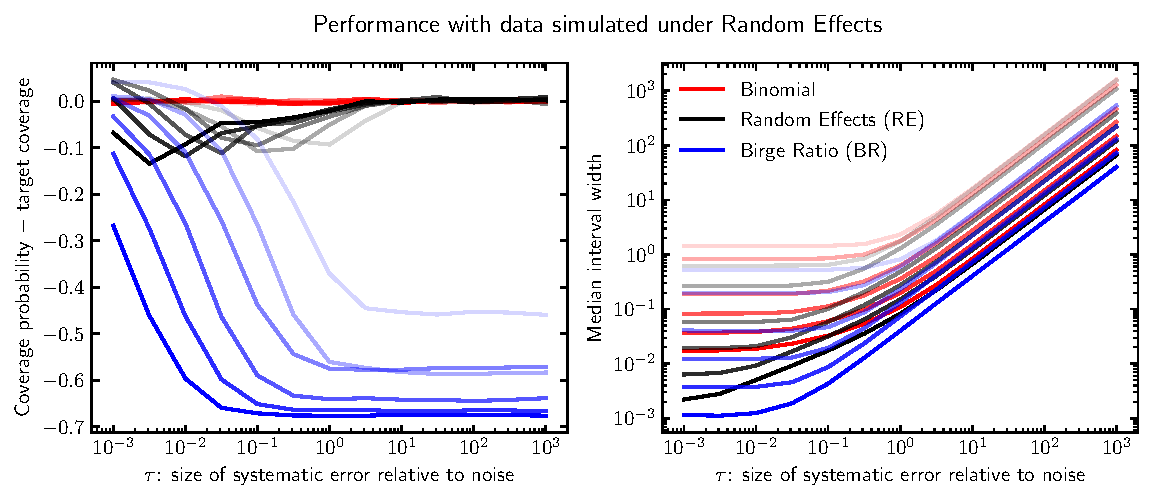
\includegraphics[width=\textwidth]{figs/performance_random_effects.pdf}
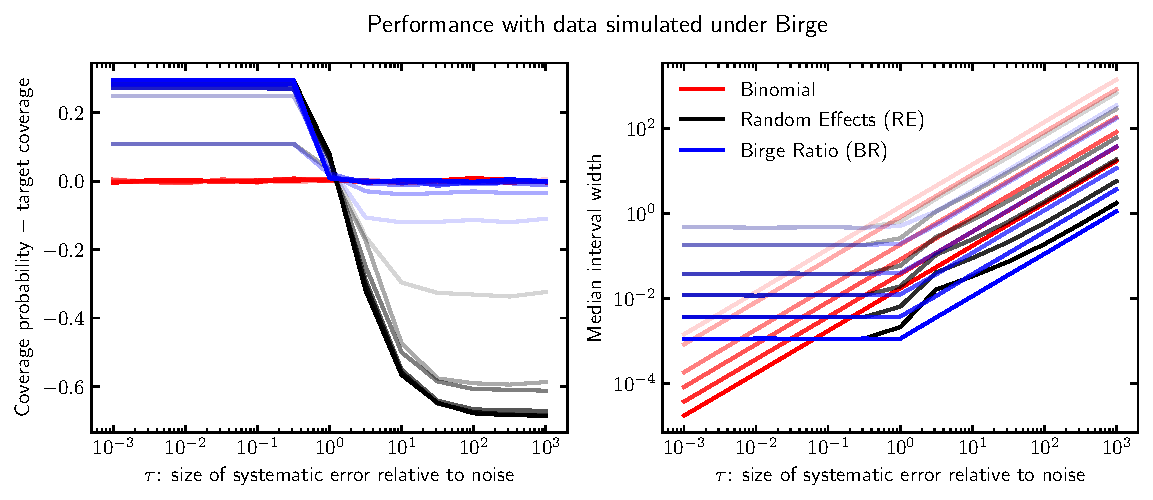
\includegraphics[width=\textwidth]{figs/performance_birge.pdf}
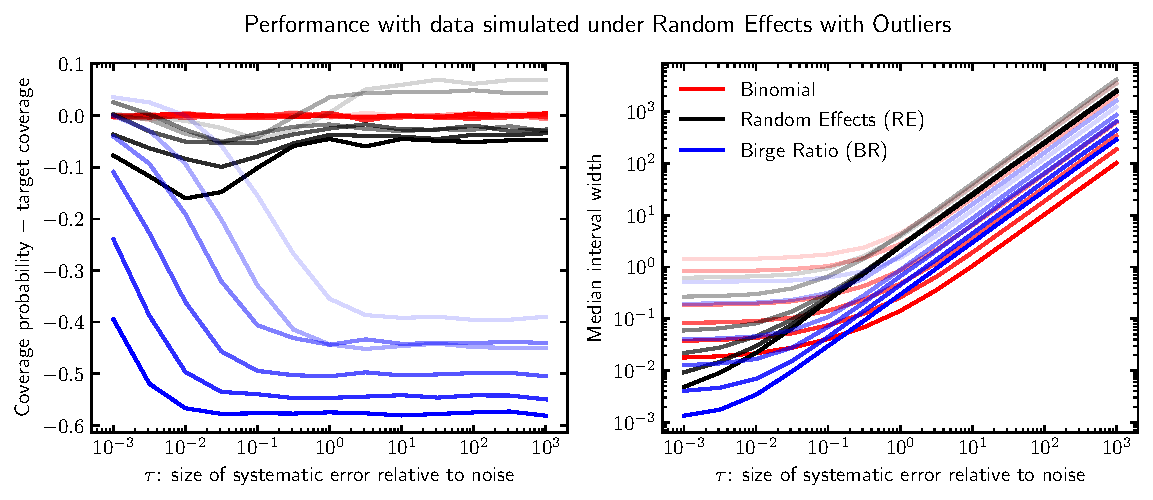
\includegraphics[width=\textwidth]{figs/performance_random_effects_outliers.pdf}
\label{fig:sim-results}
\caption{Simulation results under the three settings satisfying our assumptions. The darkest color is $n=1000$, and the lightest color is $n=3$.}
\end{figure}

We show results for the settings satisfying our assumptions (Random Effects, Birge, Random Effects with Outliers) in \ref{fig:sim-results}. Since the target coverage level is varied across simulations, we report the difference in achieved coverage and target coverage. Here are some observations.

\begin{itemize}
\item
  The Sign Test perfectly achieves target coverage in every single scenario. This is not surprising given its mathematical setup, and that every single scenario satisfies ST's assumptions.
\item
  Under the Random Effects model, RE yields better coverage with smaller intervals when the systematic errors are small, but does not achieve coverage when systematic errors are comparable to or larger than noise. This is surprising until we remember that inference for the Random Effects model is approximate, not exact. BR performs very poorly, espeially for large $n$.
\item
  Under the Birge model, note that it is slightly unrealistic to have $\tau<1$, because that implies that the $\sigma_i$'s given to us are actually \emph{overestimates} of the true standard deviation. Considering the case where $\tau\geq 1$, the BR method works well, as we would expect, though does it does not achieve target coverage when $n$ is small (as inference is approximate and not exact). BR also offers far narrower intervals than ST. RE works decently well; maintains at least target coverage, but offers larger intervals for large $n$ than Binomial and BR for roughly $\tau>3$. For context, in the gravitational constant data shown later \citep{tiesinga2021codata}, we estimate $\tau\approx 3.6$ under the Birge model.
\item
  Under Random Effects with Outliers, which satisfies the assumptions of neither RE nor BR, BR works poorly, while RE is fairly competitive with ST (though it yields intervals larger by orders of magnitude for large $n$ with $\tau>1$). This difficulty in this setting is outliers, especially at large $n$, which pull or greatly expand the RE and BR intervals. As expected, ST still achieves perfect coverage in this setting. In general, ST is robust to outliers as it only depends on the ranking of the experiments, not their relative magnitudes.
\end{itemize}

\begin{figure}[htbp]
\centering
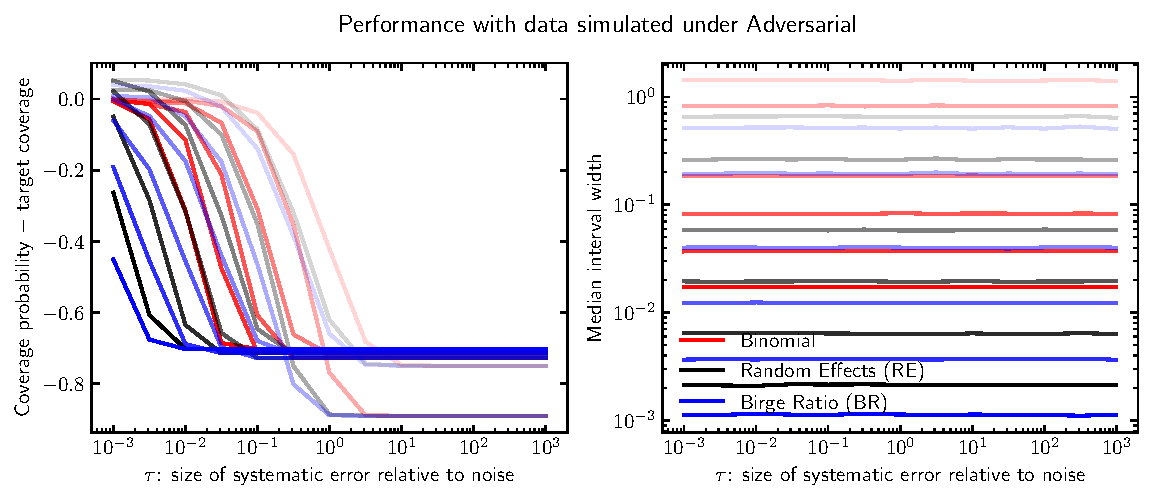
\includegraphics[width=\textwidth]{figs/performance_adversarial.pdf}
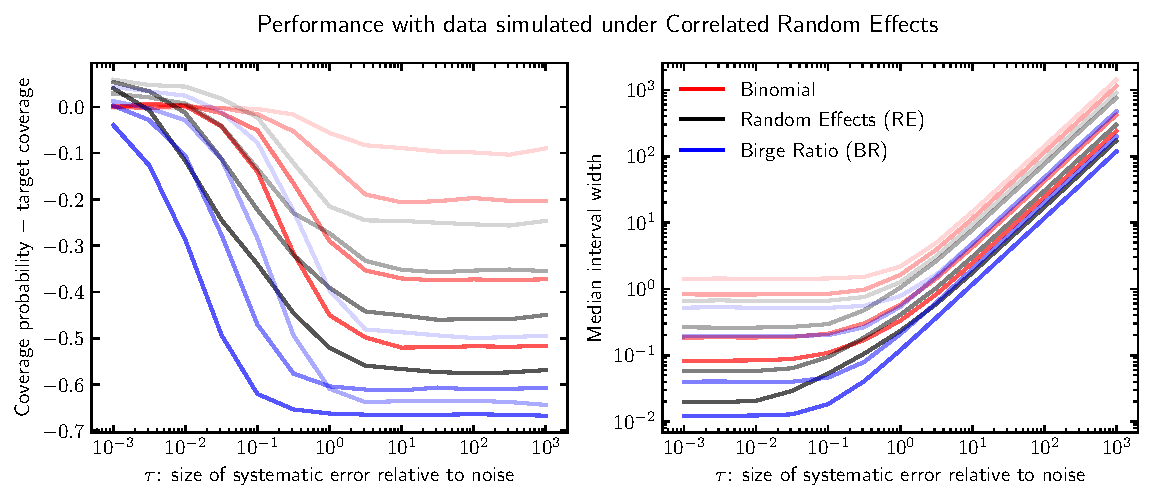
\includegraphics[width=\textwidth]{figs/performance_random_effects_corr.pdf}
\label{fig:sim-results2}
\caption{Simulation results under the two settings not satisfying our assumptions. The darkest color is $n=1000$, and the lightest color is $n=3$. Note that in the Correlated Random Effects setting, we don't do simulations for $n>100$ due to computational difficulties.}
\end{figure}



\ref{fig:sim-results2} contains results for the settings not satisfying our assumptions (Adversarial and Correlated Random Effects).

\begin{itemize}
\item
  As $\tau$ increases, the Sign Test maintains target coverage for longer than RE and BR for all values of $n$.
\item
  For small $n$, all methods are less sensitive to the these particular assumption violations.
\end{itemize}

\subsection{Simulation discussion}\label{simulation-discussion}

The main message from the simulations is that, by using nonparametric methods which ignore the $\sigma_i$'s, much robustness is gained, and (usually) little precision lost. The primary exception to this is when systematic errors are quite small and the scales of the noise vary widely. Intuitively, this is the case when the $\sigma_i$'s are most informative, and the most can be gained from using them.

But when systematic errors are large, or systematic errors are within the same order of magnitude of each other, it seems not much is gained by incorporating the $\sigma_i$ information.

This parallels results from nonparametric statistics that show nonparametric methods like the Sign Test and Signed-Rank Test don't sacrifice much efficiency over methods like a $t$-test which make stronger assumptions \citep{conover1999practical}.

\section{Real-world performance}\label{sec:realworld}

We have just performed a simulation study to examine how different methods perform under different assumed data-generating processes. However, when doing a real meta-analysis, none of the above assumed data-generating processes will be true. To get a more realistic handle on the performance of the different methods above, we can examine whether or not the different methods can recover, using old studies, values $\theta$ which now have precise knowledge of. We will use the datasets described in Section \ref{sec:historical-studies} towards this purpose.

To our knowledge, such an evaluation of meta-analysis methods has not been done before. This is not surprising, because the modern development of meta-analysis has mostly been in medicine and the social sciences, where ground truths are either too difficult to obtain or simply not well-defined (e.g.~a treatment effect will vary between different populations, so what would the ``ground truth'' treatment effect be?). In the physical sciences, in contrast, it is typically easy to imagine that there is a ``ground truth,'' and the improvement in techniques over time can offer improvements of orders of magnitude in our uncertainty about it.

Note that, because of the same differences that make this study possible in the physical sciences but not in social science and medicine, this section's results cannot automatically be applied to meta-analysis in social science and medicine.

\subsection{Particle Data Group, 1970}

This is the dataset shown in Figure \ref{fig:particle}. We have enough data here to take quite a close, quantitative look at the performance of the different methods. This is how we shall proceed:
\begin{enumerate}
  \item For a given $n$, consider all particle properties with $N\geq n$ results.
  \item For a given particle property, there are $\binom{N}{n}$ possible combinations of $n$ results. Each combination forms a dataset of $n$ results with a corresponding ground truth.
  \item For each of the combinations (or a random sampling of them if there are many), we can apply the methods, and compute various statistics. For the purposes of this section, the interval yielded by a method ``contains the ground truth'' if it overlaps with the 2025 $2\sigma$ interval for the corresponding particle property.
  \item Average first over the combinations within each particle property, then over the particle properties. (If we averaged over all combinations together, datasets with large $N$ would dominate the others in the results for small $n$ values).
\end{enumerate}
This way, for our evaluation at, say, $n=3$, we can use datasets like \texttt{M018W1} with many more than 3 results. Thus our conclusions for any $n$ will be based on a larger and more varied set of datasets and will be more robust.

\begin{figure}[htbp]
  \includegraphics[width=\textwidth]{figs/pdg1970_cov_birge.pdf}
\caption{
Top: Coverage comparison of the different variations of the Birge Ratio method discussed in Section \ref{sec:birge} on the 1970 PDG dataset, with the Fixed Effect result for reference. Bottom: Average width of intervals from the different methods compared to Fixed Effect. None of the methods achieve target coverage for any value of $n$, and coverage decreases as $n$ increases.
}\label{fig:pdg1970-cov-birge}
\end{figure}

Figure \ref{fig:pdg1970-cov-birge} shows the coverage achieved by the Birge Ratio and PDG's and CODATA's variations on it:
\begin{itemize}
  \item None of Birge Ratio methods achieve target coverage for any $n$. In this experiment, target coverage is $0.6827$ ($1\sigma$), and coverage for all the methods drops below $0.4$ for $n=10$. Coverage is quite close to target for the standard method and PDG's for $n$ from 2 to 3.
  \item Among the variations on the Birge Ratio, PDG offers the highest coverage. This is perhaps unsurprising, as their heuristic to exclude high-$\sigma_i$ data when fitting the scaling factor is designed for their dataset, where experiments may sometimes have $\sigma_i$'s at different orders of magnitude.
  \item For small $n$, CODATA's heuristic for choosing the scaling factor results in intervals almost as narrow as those from Fixed Effect. This is because their heuristic is to scale the $\sigma_i$'s up until the largest is at most $2\sigma_i$. For small $n$ and a moderate scaling factor $c$ (say, $c=1.5$), we are unlikely to have any residuals above $2\sigma_i$ ($1.33c\sigma$), so we will not scale and will simply yield a Fixed Effect estimate.
\end{itemize}

\begin{figure}[htbp]
  \includegraphics[width=\textwidth]{figs/pdg1970_cov_re.pdf}
\caption{
Top: Coverage comparison of the different variations of the Random Effects method discussed in Section \ref{sec:re} on the 1970 PDG dataset, with the Fixed Effect result for reference. Bottom: Average width of intervals from the different methods compared to Fixed Effect. We see that coverage decreases as $n$ increases.
}\label{fig:pdg1970-cov-re}
\end{figure}

Figure \ref{fig:pdg1970-cov-re} shows results for a few methods for Random Effects inference:
\begin{itemize}
  \item For $n>2$, none of Random Effects methods achieve target coverage. In this experiment, target coverage is $0.6827$ ($1\sigma$), and coverage for all the methods drops below $0.6$ and then below $0.5$ for $n=10$. Coverage is quite close to target for the DL and HKSJ for $n$ from 2 to 3.
  \item Surprisingly, HKSJ holds no clear advantage in coverage over DL, even though (as expected) it tends to yield wider intervals.
\end{itemize}

\begin{figure}[htbp]
  \includegraphics[width=\textwidth]{figs/pdg1970_cov_nonparam.pdf}
  \caption{
Coverage comparison of the nonparametric methods presented in Section \ref{sec:methods} on the 1970 PDG dataset. Solid lines are achieved coverages, dashed lines are target coverages---these vary with $n$ due to the discreteness of the methods. ST: Sign Test. SRT: Signed-Rank Test. ST$_{\rho=0.1}$ indicates the Sign Test with the CDF modified to accomodate the events $(y_i>\theta)$ and $(y_j>\theta)$ having correlation $\rho=0.1$. ST and SRT both under-cover, though SRT is better. Incorporating correlation using ST$_\rho=0.1$ yields coverage exceeding or closer to matching its target. The overlap between ST and ST$_\rho=0.1$ for n from 3 to 7 is because both methods yield intervals based on quantiles of the points. For $n=3$, they will yield the same interval from the smallest value to the biggest value, and therefore achieve the same coverage, but ST will call it a 75\% interval and ST$_\rho=0.1$ will call it a 67.5\% interval.
}\label{fig:pdg1970-cov-nonparam}
\end{figure}


Figure \ref{fig:pdg1970-cov-nonparam} shows results for the Sign Test (Section \ref{sec:st}), Signed-Rank Test (Section \ref{sec:srt}), and the Sign Test modified to allow for correlations between the results. We see that both the Sign Test and the Signed-Rank Test consistently under-cover (i.e.~they do not contain the ground truth value as often as they should if their assumptions are true). Interestingly, even though its assumptions are stronger, the Signed-Rank Test performs better, with gaps in coverage of at most about 0.05. We also see that the correlation-modified Sign Test at times exceeds its target coverage and never falls nearly as far short of its target as the Sign Test, pointing towards the possible practical utility of this modification.

\section{Results on real data}\label{results-on-real-data}

\subsection{CODATA: physical constants}\label{codata-physical-constants}

We ought to run a comparison on some real data. Let's see what happens with CODATA (Committee on Data of the International Science Council) estimates of physical constants. Because physical constants aren't known exactly, we don't have a ground truth, but we can at least see the behavior of the different methods with real experimental data.

\subsubsection{Gravitational constant}\label{gravitational-constant}

\begin{figure}[htpb]
\centering
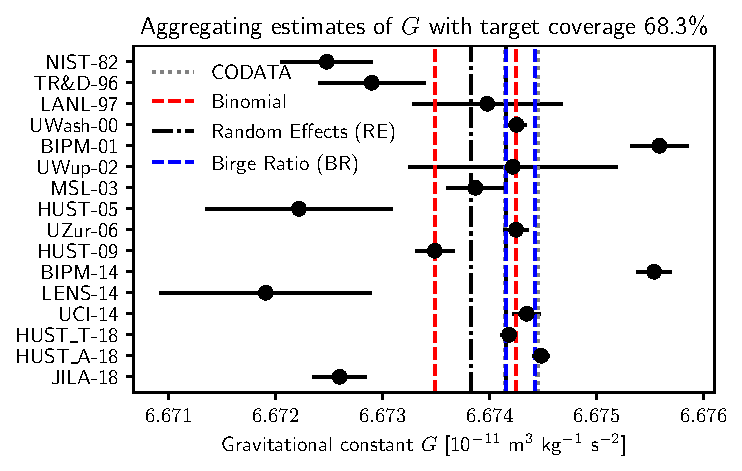
\includegraphics[width=0.5\textwidth]{figs/G0.pdf}
\label{fig:G}
\caption{Results of different aggregation methods for estimates of the gravitational constant $G$ \cite[Table XXIX]{tiesinga2021codata}. Error bars are $1\sigma$ intervals using the $sigma_i$'s reported by each study.}
\end{figure}


We get data from 16 experiments estimating the gravitational constant $G$ from the 2018 CODATA adjustment \citep[Table XXIX]{tiesinga2021codata}. Results are shown in \ref{fig:G}. Note that for $n=16$, the nominal coverage level of the Binomial interval is $0.7900$. The nominal coverages of the other intervals under their respective models are $0.6827$.

We see that the CODATA interval is slightly wider than that given by our application of BR. CODATA uses BR too, but there are two differences:

\begin{itemize}
\item
  They take into account small correlations between some pairs of experiments.\footnote{(NIST-82, LANL-97), (HUST-05, HUST-09), and (HUST-09, HUST$_\text{T}$-18) are correlated \citep{tiesinga2021codata}.}
\item
  Their inference on $\tau$, effectively the expansion factor for the $\sigma_i$'s is heuristic, and they choose $\tau=3.9$ to ``decrease the residuals to below two'' \citep{tiesinga2021codata}.
\end{itemize}

The CODATA and BR intervals are pulled to the right by the small $\sigma_i$'s on many of the rightmost points. The RE interval is just about disjoint with the CODATA and BR intervals---this is because it models systematic errors additively, rather than multiplicatively. The Binomial interval is wider than any of the other intervals. Note how it is supported by the HUST-09 and UZur-06 points, and has 5 points outside it on its left, and 5 points outside on the right.

\subsubsection{Planck constant}\label{planck-constant}

\begin{figure}[htpb]
\centering
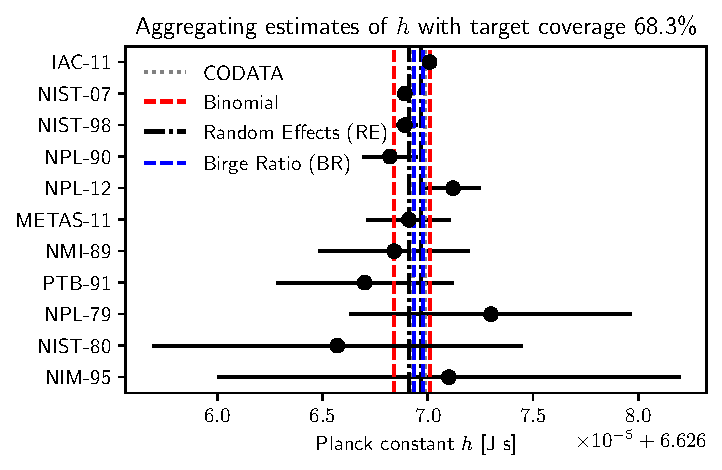
\includegraphics[width=0.5\textwidth]{figs/h0.pdf}
\label{fig:h}
\caption{Results of different aggregation methods for estimates of the Planck constant $h$ \cite[Table 26]{mohr2012codata}. Error bars are $1\sigma$ intervals using the $sigma_i$'s reported by each study.}
\end{figure}

We get data from 11 experiments estimating the Planck constant $h$ from the 2010 CODATA adjustment \cite[Table 26]{mohr2012codata}.\footnote{Since the 2019 SI unit redefinition, the SI units are defined, in part, based on the Planck constant, so there is no longer ``uncertainty'' in it in terms of SI units. But the dataset still offers an interesting case study.}

Results are shown in \ref{fig:h}. Note that for $n=11$, the nominal coverage level of the Binomial interval is $0.7734$. The nominal coverages of the other intervals under their respective models are $0.6827$.

We see again that the CODATA interval is wider than that given by our BR---this is because CODATA take into account some correlations between data points. In the Planck constant data, the BR interval is contained within RE, and RE is contained with the Binomial interval. We see that the Binomial interval is supported by points NMI-89 and IAC-11, with 3 points lying outside to either side.

\subsection{Targeting the same coverage level on real data}\label{targeting-the-same-coverage-level-on-real-data}

\begin{figure}[htbp]
\centering
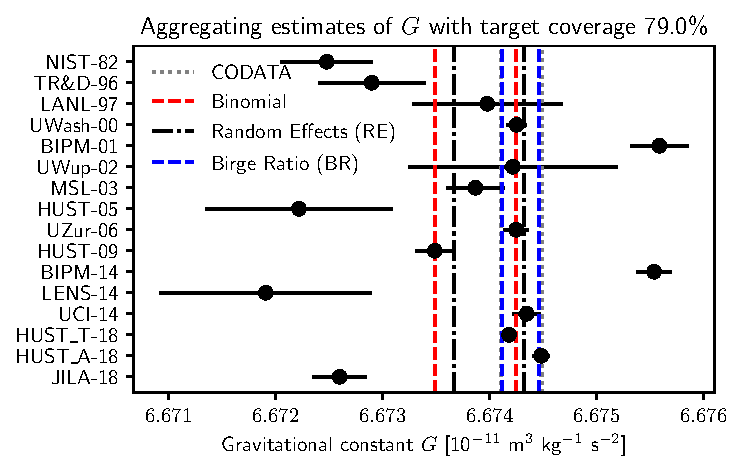
\includegraphics{figs/G1.pdf}
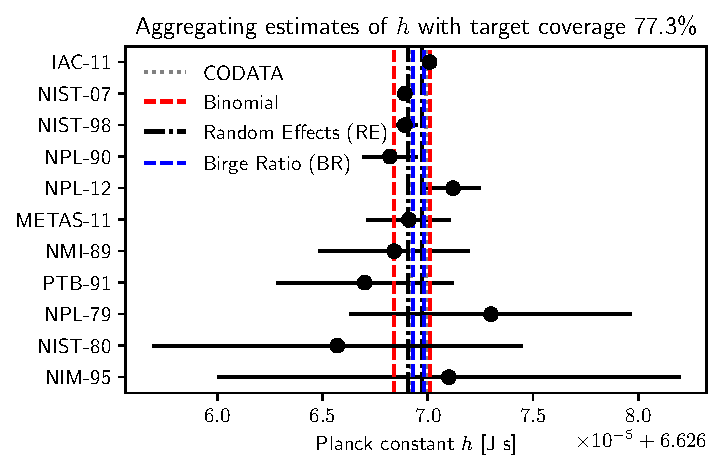
\includegraphics{figs/h1.pdf}
\label{fig:Gh-wider}
\caption{Since the Sign Test can target only a discrete set of coverages, for the $G$ data it will (under the assumptions) achieve coverage 79.0\%, and 77.3\% for the $h$ data. For comparison, in this figure the intervals from CODATA, RE, and BR are expanded to target these coverage levels. The CODATA, RE, and BR intervals from \ref{fig:G} and \ref{fig:h} have been scaled them by the corresponding $z_{\alpha/2}$.}
\end{figure}

\section{Case study: Fundamental particles}\label{case-study-fundamental-particles}

\section{Case study: Ice sheet mass balance}\label{case-study-ice-sheet-mass-balance}

\section{Discussion}\label{discussion-2}

\subsection{Is unaccounted-for error additive or multiplicative?}
A significant tension in the literature is whether unaccounted-for errors should be modeled as additive (true variance is $\sigma_i^2+\tau^2$) or multiplicative (true variance is $c^2\sigma_i^2$). The physics literature tends to favor the multiplicative model and its corresponding Birge Ratio method(s), while the meta-analysis literature as a whole favors the additive model and Random Effects method(s). Here is a summary of our results:

\begin{itemize}
  \item In Section \ref{sec:assumptions}, every analysis and model comparison on almost every dataset favors the Random Effects model, including datasets from the Particle Data Group and datasets with or without ground truths. There is no obvious difference between the physical and non-physical datasets.
  \item In Section \ref{sec:simulation}, the Birge Ratio method does not work well on data from Random Effects, but Random Effects works well on data from the Birge Ratio.
  \item In Section \ref{sec:realworld}, we see that the Random Effects method is closer to achieving coverage on the 1970 PDG dataset than the Birge Ratio is.
\end{itemize}
So every sign points towards Random Effects being better than the Birge Ratio, both in terms of the validity of its assumptions and in terms of actual performance in inference.

\subsection{Nonparametric methods for meta-analysis}
In Sections \ref{sec:st} and \ref{sec:srt}, we introduced for the first time inversions of the Sign Test and Signed-Rank Tests as methods for meta-analysis. These have some good properties in this setting:
\begin{itemize}
\item Make weaker assumptions which are implied by many existing common assumptions.
\item Yield confidence intervals which exactly achieve their nominal coverage level for any value of $n$ and for any data-generating process which satisfies the relatively weak assumptions.
\item Are insensitive to problems in the $\sigma_i$ uncertainties provided for each underlying estimate.
\item Are robust to outliers, because they don't make a light-tailed distributional assumption.
\end{itemize}
In addition, the Sign Test in particular relies on fairly simple math, making its justification, implementation, and interpretation easy for non-statisticians.

In Sections \ref{sec:simulation} and \ref{sec:realworld}, we saw that both of these methods yield intervals which more consistently achieve the desired level of coverage than others. Of course, this comes at the cost of wider intervals, but this is partly because the intervals given by other methods are just unrealistically narrow.

However, both of these methods have some limitations:
\begin{itemize}
\item Even though they can exactly achieve some coverage levels, neither can exactly achieve an arbitrary target coverage level for finite $n$ due to the discreteness of the underlying distributions. This problem is much worse for the Sign Test than for the Signed-Rank Test. Though we do discuss in Section \ref{sec:st} some approaches to mitigate it.
\item Both will yield wider intervals than needed if we know more about the data-generating process---methods tailored to that DGP can achieve coverage with narrower intervals. Though we demonstrate in Section \ref{sec:simulation} that, in many cases, the gain is not much.
\item Neither takes advantage of the information present in the $\sigma_i$'s.
\item Even the weaker assumptions made by these methods do not hold in real-world data. In particular, in Section \ref{sec:historical-assumptions-check}, we were able to detect violations of the independence assumption in a real-world dataset. However, as we demonstrate in Sections \ref{sec:simulation} and \ref{sec:realworld}, this can accomodated with a small modification to the Sign Test.
\end{itemize}

\section*{Acknowledgements}

The parts of this study relying on real-world data incorporate thousands of scientific results obtained by thousands of authors. Though we cannot cite them all, this work would not have been possible without them.

We thank Dean Robinson and Ben Nachman for helpful communication about PDG data, and the PDG as a whole for their carefully documented datasets and machine-readable data. We also thank Rose Baker for providing the datasets from \citet{baker2013meta}.

\twocolumn
\footnotesize
\bibliography{references}
\normalsize

\end{document}